%! TEX root = ../main.tex
\chapter{Propuesta de solución}
\label{chap:solucion}


Descriptos los fundamentos teóricos del uso de videojuegos serios en el ambiente
educativo, sobre todo en aquellas áreas que requieren más practica para la
adquisición de la pericia necesaria, e identificando el área de enfermería como
uno de estas se definieron las problemáticas actuales de la educación de
enfermeros y seleccionamos algunos procedimientos que serán utilizados para el
contenido de la solución. A continuación se busca converger todos los aspectos
descriptos en capítulos anteriores.

La solución propuesta en este trabajo consiste en el desarrollo de una
aplicación para dispositivos móviles que se define como un juego serio llamado
\Gls{yave}, basado en el construccionismo, el cual incluye conceptos de la
gamificación, y de simulación. El juego consiste en ofrecer a los usuarios, en
este caso alumnos de enfermería, un medio en el cual puedan realizar
procedimientos de enfermería y cuyo objetivo es servir como herramienta de apoyo
en el aprendizaje.

\Gls{yave} permitirá al usuario poder seleccionar el procedimiento que quiera
realizar, en cada procedimiento se le dará la posibilidad de interactuar con un
paciente y con una conjunto de objetos que forman parte de las herramientas
requeridas para realizar el procedimiento seleccionado. Además, contempla la
posibilidad de realizar acciones relacionadas a la bioseguridad, y otros 
aspectos transversales a la educación de un enfermero.

La solución no solo le permitirá al usuario realizar los procedimientos para
poner en practica sus conocimientos sobre el mismo, sino también evaluará al
usuario, dándole al final de cada sesión una puntuación y describiendo los
pasos realizados correcta e incorrectamente, proporcionando información acerca
de los puntos incorrectos.


%%! TEX root = ../main.tex


\section{Acciones condicionadas por eventos}

Un evento es la ocurrencia de un hecho en particular, y son identificados por un
nombre y un conjunto de parámetros, por ejemplo, cuando un evento es cuando el
enfermero inserta una Jeringa, el nombre de este evento es
\emph{''jeringa.inserted''}, y sus parámetros podrían ser el lugar y el tiempo
de la inserción, así, la influencia del estudiante en la simulación es una
sucesión de eventos.

Por cada acción que realiza el usuario dentro de la simulación, existe un evento
relacionado, por consiguiente, es razonable estudiar algunos eventos para
determinar si los pasos realizados corresponden con los deseados. 

Para determinar si una sucesión de eventos es la correcta, se definen reglas,
una regla es una asociación de una condición y una acción, la condición define
si el entorno es el adecuado para realizar una acción, la cual es un
procedimiento que realiza la lógica deseada.

Las \gls{eca} son aquellas que son activadas una vez que se cumplen determinados
eventos\cite{bailey2004event}. En las bases de datos relacionales, son conocidos
como triggers, es decir, una base de datos relacional (u orientada a objetos) es
un motor de reglas \gls{eca}\cite{bailey2004event}\cite{behrends2006combining}.

Las mismas pueden ser utilizadas para notificar que un determinado conjunto de
eventos ha ocurrido\cite{bailey2004event}, así como servir para almacenar
información acerca de la utilización de un determinado recurso.


\subsubsection{Motivación}

Las reglas del tipo \gls{eca} permiten reaccionar a determinados eventos, en
forma de una única regla, la cual facilita la declaración de las
mismas\cite{bailey2004event}.

Son principalmente útiles para analizar el comportamiento en tiempo real de un
sistema en una forma
reactiva\cite{bailey2004event}\cite{de2001eca}\cite{bailey2002analysis}, esta
característica esta impulsada principalmente por que son ejecutadas después de
la ocurrencia de un evento, y el entorno no es modificado, pudiendo así acceder
al mismo entorno que el qué lanzo el evento.

Definir si las acciones de un usuario son correctas utilizando un motor
\gls{eca} es sencillo desde el punto de vista que sólo se deben definir un
conjunto de acciones que se deben realizar, y agregar una acción que verifica si
los pasos realizados fueron los correctos.

\subsection{Declaración}

Una \gls{eca}, se define como\cite{bailey2004event}\cite{behrends2006combining}:

\begin{center}
	 Cuando ocurren una serie de \emph{eventos}, y se cumple una
	 \emph{condición}, entonces realizar una \emph{Acción}.
\end{center}

Los \emph{eventos} determinan cuando una regla debe ser activada, los mismos se
dividen en dos categorías\cite{behrends2006combining}, primitivos y compuestos,
los primeros son detectables, por ejemplo, cuando se inserta una jeringa, y los
compuestos, son la combinación de uno o más
primitivos\cite{bailey2004event}\cite{behrends2006combining}. Los eventos
compuestos, se unen mediante:
\begin{enumerate*}[label=\itshape\alph*\upshape)]
\item conjunción (\emph{y}),
\item disyunción (\emph{o}), y
\item secuencia (\emph{entonces}).
\end{enumerate*}
Sin embargo, no siempre son necesarios todas las posibles combinaciones, y las
combinaciones sencillas son más fáciles de optimizar y
probar\cite{bailey2004event}.

La \emph{condición} de una regla determina si el entorno es el necesario para que la
regla sea activada, en esta condición el entorno que lanzó el evento esta
disponible.

La \emph{acción} a ejecutar describe la lógica que debe ser ejecutada cuando se han
lanzado los eventos y la condición de la regla se ha cumplido.

\subsubsection{Dependencia entre reglas}

Las reglas pueden depender de otras reglas, lo cual se puede ver como que la
finalización de una regla es un evento que otra regla espera para poder ser
activada.

Las reglas pueden agregar información a un contexto compartido por todas las
reglas, de esta manera, se puede pasar parámetros entre distintas reglas, por
ejemplo, la regla \emph{Retirar Torniquete}, depende de la regla \emph{Insertar
Torniquete}, pero debe responder solamente al torniquete que ha activado
la regla de inserción, es decir, el usuario puede extraer varios torniquetes, y
la regla no debe activarse, hasta que se extraiga el torniquete que activo la
primer regla.

Así, la regla \emph{Retirar Torniquete} depende de la regla \emph{Insertar
Torniquete}, y esta relación entre reglas, se da en dos
formas\cite{bailey2004event}:

\begin{itemize}
\item  \emph{Dependencia fuerte:} la regla \emph{Retirar Torniquete} solamente podrá
	ser elegida para ser lanzada cuando la regla \emph{Insertar Torniquete}
	haya sido cumplida.
\item  \emph{Dependencia de contexto}: la regla \emph{Retirar Torniquete} no se
	activará cuando los eventos a los que escucha se terminen, sino cuando
	los eventos a los que escucha sean lanzados con los parámetros adecuados
	(se extraiga el torniquete que lanzo la regla de inserción).
\end{itemize}

\subsubsection{Definición}

La definición de las reglas se realiza de la siguiente forma;
\begin{algorithm}[H]
\caption{Creación de regla de verificación de calzado de guantes}
\label{alg:rule:guante}
\lstset{style=sharpc}
\begin{lstlisting}
Rule.New("Regla de verificacion de calzado de guantes").
     When("enfermero.guantes.calzar").
     Then(e => e.Patient.ManosLimpias()).
\end{lstlisting}
\end{algorithm}
%TODO agregar indice de algoritmos

La regla anterior controla que el estudiante ha realizado la acción ``Calzarse
los guantes'', y en ese momento tenga las manos limpias, la variable \emph{e},
es el entorno, y a través de la propiedad \emph{Patient} obtiene el estado del
paciente en ese momento.

\subsection{Modelo de ejecución}

Para ejecutar un motor de reglas del tipo \gls{eca}, se debe tener en cuenta
principalmente dos factores, 
\begin{enumerate*}[label=\itshape\alph*\upshape)]
\item  Como se verifica el cumplimiento de cada regla, y, 
\item  Que ocurre cuando varias reglas son lanzadas al mismo tiempo
\end{enumerate*}.

Para ambos casos se puede tomar un enfoque \emph{inmediato}, es decir que
inmediatamente cuando se lanza un evento, o se cumple una condición, se ejecuta
la regla. Además existen otros dos modos de ejecución, \emph{deferida}, y
\emph{desacoplada}, en la primera, se espera hasta que el lanzador del evento
culmine su trabajo, y luego se ejecuta la regla, pero en la misma unidad de
trabajo, mientras que en la ejecución desacoplada, se encolan los trabajos y
otro hilo es el encargado de ejecutar las reglas. Estos modos están inspirados
en las bases de datos relacionales, el deferido se ejecuta en la misma
transacción, y el desacoplado, inmediatamente después de que la transacción
termine\cite{bailey2004event}.

La propuesta implementada, utiliza una ejecución inmediata, principalmente por
la sencillez de las reglas, es decir, las reglas no realizar un proceso complejo,
solamente controlan el estado del entorno y lo validan.

Además, la ejecución inmediata es importante por que el entorno no sufre
modificaciones entre el evento lanzado y la ejecución de la regla, según
\cite{bailey2004event}, este es el factor más importante para determinar el tipo
de ejecución deseado.



\subsubsection{Estados de una regla}

Una regla puede estar en uno de los siguientes estados:

\begin{description}
\item[BEGIN] Es una regla que recién fue creada, no realiza ninguna
	acción.
\item[WAITING\_FOR\_RULE] Es un estado en el que esta esperando que otras reglas
	sean lanzadas. En este estado, es un suscriptor de las reglas por la que
	espera, y no forma parte del ciclo de ejecución del motor de reglas.
\item[WAITING\_FOR\_EVENT] Es un estado en el que esta escuchando a que sean
	lanzados los eventos a los que escucha, este es el estado principal. En
	este estado, es un suscriptor de los eventos por los que espera, y no
	forma parte del ciclo de ejecución del motor de reglas. Se diferencia
	del estado anterior, en que los eventos escuchados pueden ser lanzados
	por cualquier objeto del entorno, no necesariamente una regla.
\item[WAITING\_FOR\_CONDITION] La regla ya no espera por ningún evento y las
	reglas de las que depende ya han sido lanzadas, se verifica cada cierto
	tiempo si el entorno cumple con una condición definida. 
\item[FINISH] La regla ha sido lanzada, con un resultado no determinado, se pudo
	haber cumplido, como no, es el estado final de una regla. Cuando una
	regla llega a este estado, se lanza su evento de finalización.
\end{description}

Una regla puede estar en solo un estado, y solamente se permite que el estado
avance, desde \emph{BEGIN} hasta \emph{FINISH}.


\subsubsection{Ciclo de vida}

Cuando una regla es definida, y insertada al motor de reglas, inmediatamente
pasa al estado \emph{BEGIN}, luego se verifica si la misma depende de otras
reglas, sí este es el caso, pasa al estado \emph{WAITING\_FOR\_RULE} y escucha a
los eventos de finalización de las reglas anteriores.

Una vez que las reglas anteriores han sido finalizadas, la regla pasa al estado
\emph{WAITING\_FOR\_EVENT} sí deben escuchar por algún evento, en caso contrario
pasan al estado \emph{WAITING\_FOR\_CONDITION}.

Una vez que la regla está en estado \emph{WAITING\_FOR\_CONDITION}, pasa a un
motor que ejecuta su condición cada cierto tiempo, si la condición se cumple, la
regla se ejecuta, y la misma pasa a estado \emph{FINISH}, momento en el cual
notifica a las reglas que dependen de ella que ha sido lanzada.

Una vez que la regla esta en estado \emph{FINISH}, la misma sale del esquema de
ejecución, y solo esta disponible para obtener resultados.

Según el ejemplo de la regla definida en el código \ref{alg:rule:guante}, la
regla al terminar de ser construida pasa a estado \emph{BEGIN}, al no depender
de otras reglas, pasa inmediatamente al estado \emph{WAITING\_FOR\_EVENT},
cuando es lanzado el evento, la regla ejecuta la acción y pasa al estado
\emph{FINISH}.

\subsubsection{Motor de ejecución}

Un motor de reglas \gls{eca}, requiere de un proceso que evalúe constantemente
las reglas para verificar si las mismas deben ser lanzadas o
no\cite{bailey2004event}\cite{galton2002two}, este motor puede utilizar el
algoritmo de RETE\cite{de2001eca} para realizar esta verificación, en la
propuesta presentada, la cantidad de reglas definidas, y la no dependencia
circular entre ellas, hace innecesario la implementación de tal
algoritmo\cite{de2001eca}. 

El motor de reglas actúa sobre aquellas reglas en estado
\emph{WAITING\_FOR\_CONDITION} e invoca al procedimiento que se encarga de
validar si la regla puede ser activada (el procedimiento es único por cada
regla), si el mismo determina que la regla puede ser lanzada, el motor ejecuta
la acción de la regla y modifica el estado de la regla a \emph{FINISH}.

%! TEX root = ../main.tex
\section{Tecnologías disponibles}

Para el desarrollo de videojuegos se utilizan programas o herramientas
especializadas en ello llamadas \enquote{Motores de videojuegos}. A continuación
se da una breve introducción de lo que es un motor de videojuego o motor
gráfico.

El término \enquote{motor gráfico} o \enquote{motor de videojuegos} hace
referencia a una serie de rutinas de programación que permiten el diseño, la
creación, el desarrollo y la representación gráfica de un
videojuego\cite{videojuego:telechea}.

Además, la gran mayoría de estos motores ofrecen a su vez características y
funciones que facilitan la construcción del videojuego, como el motor físico
(software capaz de realizar \enquote{simulaciones} de ciertos sistemas físicos
como la dinámica de un cuerpo rígido, el movimiento de un fluido o la
elasticidad) o detector de colisiones, sonidos, \textit{scripting}, animaciones,
inteligencia artificial, comunicación a través de redes, \textit{streaming},
administración de memoria, etc\cite{videojuego:telechea}.

El motor de juego utilizado depende de las características que posea el
videojuego que se quiere desarrollar. Por lo mismo, a continuación se da una
breve descripción de los motores más utilizados actualmente, se definen los
criterios para de selección y se realiza una comparación entre los mismos, y se
define el motor que más se adecue a las necesidades.

\subsection{Unreal Development Kit}

\textit{Unreal Engine} es el motor de juegos desarrollado por \textit{Epic
    Games}, se ofrece bajo un plan de suscripción mensual. El servicio de
suscripción permite a los desarrolladores unirse a una comunidad dedicada a la
construcción de grandes juegos y evolución del \textit{Unreal
    Engine}\cite{unrealengine}.

\textit{Unreal Engine} permite desarrollar juegos para plataformas como
\textit{Windows PC, Mac, iOS y Android}. También es compatible con \textit{Xbox
    One} y \textit{PlayStation 4}. Existen además trabajos recientes sobre otras
plataformas como \textit{HTLM5} y \textit{Linux}\cite{unrealengine}.

Sin embargo existe una versión gratuita del \textit{Unreal Engine}, el
\Gls{udk}. El \Gls{udk} es la edición gratuita de \textit{Unreal Engine
    3}\footnote{Versión previa a la actual versión comercial.} que proporciona
acceso al motor de juegos 3D y a la herramienta profesional que se utiliza en el
desarrollo de videojuegos \textit{blockbuster}, visualización arquitectónica, el
desarrollo de juegos para móviles, modelos 3D, películas digitales y más.
Utilizando \Gls{udk} se pueden implementar juegos y aplicaciones en
\textit{Windows PC}, \textit{iOS} y \textit{Mac}.


\subsection{Blender Game Engine}

\enquote{Blender Game Engine} es el motor de juego de \textit{Blender
    Foundation} que permite crear aplicaciones 3D interactivas o simulaciones,
desarrollabo bajo la licencia \Gls{gnu}. La principal diferencia entre el
\textit{Blender Game Engine} y el Blender convencional está en el proceso de
renderizado\cite{blender}.

Es importante no confuir con \textit{Blender}, pues este es un software de
modelado \textit{3D} y animaciones, pero esto se renderiza fuera de linea, es
decir, una vez generadas no pueden ser modificadas. Por el contrario
\textit{Blender Game Engine} genera las escenas de forma continua en tiempo real
e incorpora facilidades para la interacción del usuario durante el proceso de
\textit{renderización}\cite{blender}.

Procesa la lógica de sonido, de la física y la representación de simulaciones en
orden secuencial. El motor esta escrito en \textit{C++}. Posee un editor que
proporciona una profunda interacción con la simulación, su funcionalidad se
puede ampliar con \textit{scripts} \textit{Python} y esta diseñado para abstraer
las características complejas del motor en una interfaz de usuario simple, que
no requiere programación\cite{blender}.

El motor de juego puede simular contenido dentro de \textit{Blender}, sin
embargo, también incluye la posibilidad de exportar en plataformas como
\textit{Windows, Linux y Mac OS}. También hay soporte básico para plataformas
móviles con el proyecto \textit{Android Blender Player GSOC 2012}.

\subsection{CryEngine 3}

\enquote{CryEngine 3} es el motor de juegos desarrollado por \textit{Crytek}.
\textit{CryEngine} es un motor avanzado para el desarrollo de juegos, películas,
simulaciones de alta calidad y aplicaciones interactivas. Tiene características
diseñadas específicamente para \textit{Windows PC, PlayStation 3 y Xbox
    360}\cite{cryengine}.

Existe una versión gratuita de \textit{CryEngine}, denominada \enquote{CryEngine
    Free SDK} con todas las funcionalidades, esta versión esta disponible para
su descarga, pero ya ha sido descontinuada\cite{cryengine:sdk}.

\textit{CryEngine} posee además un conjunto de herramientas utilizadas para el
análisis de rendimiento\cite{cryengine}, además de un \Gls{ide}, que permite
editar texturas, interacciones, vehículos, etc.

\subsection{ShiVa3D}

\textit{ShiVa3D} es un paquete para el desarrollo de juegos y aplicaciones 3D,
posee un \Gls{ide} \Gls{wysiwyg} potente\cite{shiva}.

\textit{ShiVa} puede exportar juegos y aplicaciones para más de $20$ plataformas
de destino, incluyendo móviles como \textit{iOS, Android, BlackBerry y Windows
    Phone}, de escritorio como \textit{Windows, Mac OS X y Linux}, los
navegadores web con soporte \textit{Flash y HTML5}, así como consolas como la
\textit{Xbox 360, PlayStation3 y Nintendo Wii}. El \Gls{ide} se ejecuta en
\textit{Windows} y \textit{Mac OS X}\cite{shiva}. 

Un producto relacionado es el \enquote{ShiVa Server}, el cual permite el
desarrollo de aplicaciones multijugador. Las carácteristicas de este servidor,
incluyen alto rendimiento, comunicación \textit{VoIp}, etc. \enquote{ShiVa
    Server} se distribuye con una licencia distinta a
\textit{Shiva3D}\cite{shiva}.

\subsection{Unity3D}

\textit{Unity}\cite{unity3d} es un motor para el desarrollo de juegos,
dearrollado por \textit{Unity Technologies}, incluye un \Gls{ide} con un un
motor de \textit{renderizado} y flujos de trabajo para la creación de contenido
3D interactivo, desarrollo multiplataforma. Además cuenta con una gran cantidad
de \textit{assets}\footnote{Un \textit{Asset} es un paquete \textit{Unity} que
    puede contener modelos, librerias, sonidos, etc.} disponibles en un
\enquote{Asset Store} y una gran comunidad donde se intercambian conocimientos.

En \textit{Unity} se pueden desarrollar de forma sencilla elementos 2D y 3D.
Posee un \Gls{ide} intuitivo y flexible, el nivel visual y de audio son de gran
calidad, un sistema de animación poderoso. 

Permite desarrollar juegos para múltiples plataformas. Entre las plataformas
móviles soportadas, encontramos a \textit{iOS, Andriod, Windows Phone 8,
    BlackBerry 10}, entre las plataformas de escritorio a \textit{Windows, Mac y
    Linux}, plataformas web como \textit{Internet Explorer, Mozzilla Firefox,
    Google Chrome}\footnote{Requiere un plugin para el navegador que está
    disponible para \textit{Windows y Mac}}, y entre plataformas de consolas a
\textit{Xbox 360, Xbox One, Wii, Wii U, Nintendo 3DS}.

La versión paga de \textit{Unity}, \textit{Unity Pro} permite además plataformas
como \textit{PlayStation 4, PlayStation 3 y PlayStation VITA}.

Debido a la alta popularidad de \textit{Unity}, un paquete fue desarrollado por
\textit{Facebook} que permite una interacción sencilla con la \Gls{api} de la
red social \textit{Facebook} en un \textit{Asset} escrito en \cs{}, este paquete
se encuentra en \textit{Asset Store} de \textit{Unity}.

\section{Selección de plataforma}
\section{Entorno de desarrollo}

La creación de la solución es un proceso complejo, el cual se compone de varios
pasos necesarios, para llevar a cabo el desarrollo completo se debe recurrir a
una gran cantidad de tecnologías, herramientas, \textit{frameworks}, y recursos.

En esta sección se describen todos las partes involucradas en el desarrollo de
la solución propuesta, con excepción del motor gráfico, el cual es descrito
en~\ref{sec:seleccion_plataforma}.

La solución se compone de dos partes, la primera es la aplicación que los
usuarios utilizan para realizar las prácticas, denominada solución, y la segunda
parte, es un servidor que se encarga de almacenar la información sobre los
usuarios de la solución y como la utilizan, denominado \textit{Backend}.

Primeramente se definen las herramientas de gestión de código, pues ellas son
utilizadas tanto por la solución como por el \textit{backend}, luego se definen
las herramientas específicas de la creación de la simulación y por último, se
citan y describen de manera breve las herramientas utilizadas por el
\textit{backend}.

\subsection{Herramientas de gestión de código}

La gestión del código fuente desarrollado como parte de esta tesis se realizo
mediante la utilización de la herramienta de control de código fuente
\textit{Git}, \textit{Git} es un software de control de versiones distrubido, de
código abierto bajo la licencia \Gls{gnu}\cite{git}.

El proveedor del servicio \textit{Git} utilizado es
\textit{BitBucket}\cite{bitbucket}, el cual almacena repositorios \textit{Git},
la principal característica y motivación por la cual se utiliza este servicio es
que el mismo permite mantener varios repositorios privados de manera
gratuita\cite{bitbucket}, de esta manera, se utilizan distintos repositorios,
específicos para cada parte del presente trabajo, un repositorio para los
documentos de las reuniones y la propuesta de tesis, un repositorio que mantiene
el código fuente del libro de la tesis, un repositorio que mantiene el código
fuente, imágenes y diferentes archivos multimedia de la solución, y finalmente
un repositorio que mantiene el código fuente del servidor que almacena los datos
de los usuario.

\subsection{Desarrollo de la simulación}

El desarrollo de la solución requiere de una variedad importante de tecnologías
aparte del motor, las herramientas descritas en esta sección complementan al
motor seleccionado y facilitan la creación de contenido.

Se utilizo el \Gls{ide} \textit{Unity Editor} para la creación de las escenas,
el \Gls{ide} \textit{MonoDevelop} y el lenguaje \cs{} para la programación de la
interacción entre los componentes de la solución.

Adicionalmente se utilizaron varias herramientas de diseño para crear
componentes 3D y 2D, \textit{Make Human} es utilizado para la creación de los
pacientes, \textit{3Ds Max} permite la creación de objetos como gazas, y otros
elementos utilizados dentro de la solución. En cuanto a los gráficos 2D, se
utilizo \textit{Photoshop}, y diversas páginas web que proveían contenido
gratuito.

\subsubsection{Unity Editor}

El \Gls{ide} de \textit{Unity} es la herramienta en la se crean los juegos o
simulaciones. Este \Gls{ide} importa todos los activos que se hayan seleccionado
y los organiza dentro de él. Permite compilar las escenas con los terrenos,
luces, audio, personajes, física, entre otros. Se puede agregar interacción a
través de \textit{scripting}. En este \Gls{ide} se puede probar y editar en
forma simultánea los juegos y desplegarlos en las plataformas
elegidas\cite{unity3d}. 

Existen cinco vistas en el editor: explorador de proyectos, inspector,
jerarquía, escena y juego. Cada una de estas vistas cuenta con las herramientas
necesarias que permiten el desarrollo del juego\cite{unity3d}.

El editor se utiliza por que es única herramienta que permite crear escenas en
\textit{Unity}, sin embargo, este \Gls{ide}, no permite la edición de código
\footnote{Existen \textit{Assets} que permiten la edición de código dentro del
    \textit{Unity Editor}, pero son pagas y de baja reputación}, por ello se
necesita un editor externo de código.


\subsubsection{MonoDevelop}

\textit{MonoDevelop} es un \Gls{ide} de código abierto, bajo la licencia
\Gls{gnu} apoyado principalmente por la comunidad \textit{Mono}. Es el \Gls{ide}
utilizado por defecto en el desarrollo de aplicaciones para \textit{Unity3D}, el
mismo soporta varios lenguajes de programación, como \cs{},
\textit{UnityScript}, y \textit{Boo}. Es un \Gls{ide} multiplataforma que
soporta \textit{Windows} al igual que \textit{Unity3D}.

Existen otros editores que pueden ser utilizados para el desarrollo del código
fuente, pero los mismos no cuentan con el mismo nivel de integración y no son
gratuítos\footnote{\textit{Microsoft Visual Studio} permite el mismo nivel de
    integración que \textit{MonoDevelop} con un \textit{plugin}, pero el mismo
    era de pago durante el desarrollo de la solución}.

\subsubsection{Lenguaje de programación}

\textit{Unity3D} utiliza versiones limitadas\footnote{La definición del lenguaje
    es la misma, pero las librerías estándar no están completas} de tres
lenguajes de programación: \cs{}, \textit{UnityScript}, y
\textit{Boo}\cite{unity:script}. Estos lenguajes son compilados y orientados a
objetos.

\cs{} es un lenguaje de programación orientado a objetos diseñado por
\textit{Microsoft}, es el lenguaje más utilizado por la comunidad, y el
subconjunto de funcionalidades implementadas en \textit{Unity3D} hace que la
mayoría de las librerías disponibles para \cs{} funcionen correctamente en
\textit{Unity3D}.

\textit{UnityScript} es un lenguaje normalmente confundido con
\textit{JavaScript}, lenguaje del que esta inspirado, una de las principales
diferencias es que \textit{UnityScript} es orientado a objetos, a través de
clases, al contrario que \textit{JavaScript} que es orientado a objetos a través
de prototipos. Otras diferencias menores con \textit{JavaScript}, es que en
\textit{UnityScript}, el nombre del archivo es el nombre de una clase implícita
que engloba el contenido del archivo\cite{us_vs_js}, por ello, las librerías
disponibles para \textit{JavaScript} no son compatibles con
\textit{UnityScript}.

\textit{Boo} es un lenguaje inspirado en \textit{Python}, desarrollado bajo la
licencia \Gls{mit}, la cantidad de librerías portables a \textit{Unity3D}
disponibles es muy limitada y la aceptación de la comunidad hacia el lenguaje es
pobre.

Otra característica interesante es que, por el orden de compilación de los
proyectos \textit{Unity3D}, los archivos \textit{UnityScript} y \textit{Boo} son
compilados antes que los \cs{}, esto provoca que, las clases
\textit{UnityScript} sean utilizables desde \cs{}, lo que no se cumple en el
caso contrario, es decir, las clases \cs{} no son accesibles desde código
\textit{UnityScript} o \textit{Boo}.

Por los criterios mencionados se selecciona a \cs{} como el lenguaje de
implementación, por ser el lenguaje con más ayuda en línea, y por que las
librerías no diseñadas específicamente para \textit{Unity3d} pueden ser
utilizadas. Otro factor que influye en la elección es la familiaridad de los
autores con lenguajes similares. 

\subsubsection{Herramientas de diseño}

Las herramientas utilizadas para crear modelos 3D son las siguientes:

\begin{itemize}
\item \textbf{MakeHuman}: es un software de código abierto bajo la licencia
    \Gls{agnu} para crear personajes humanos 3D. Es una herramienta diseñada
    para simplificar la creación de seres humanos virtuales utilizando una
    interfaz gráfica de usuario\cite{makehuman}. 
\item \textbf{3DS Max}: es un software privado de modelado 3D, que además posee
    herramientas para animación, simulación y renderización. Esta herramienta
    fue utilizada para crear objetos 3D que no fueran personajes humanos y para
    exportar modelos de un formato a otro que fuera compatible con
    \textit{Unity3D}\cite{3dsmax}.
\item \textbf{Photoshop}: es una herramienta de edición de gráficos 2D de
    \textit{Adobe}, permite la creación y edición de gráficos, es utilizada para
    la creación de iconos, botones y demás contenido 2D que forma parte de la
    solución.
\end{itemize}

\subsection{Desarrollo del \textit{backend}}

A fin de registrar las actividades del usuario, se necesita de un servidor que
almacene los datos de todos los usuarios y las actividades que estos realizan
dentro de la solución.

Este servicio debe proveer:

\begin{itemize}
    \item \textbf{Alta disponibilidad}: el servidor debe estar disponible en
        todo momento, cualquier día de la semana y a cualquier hora. Los
        requisitos de accesibilidad son estrictos, pues se necesita que los
        usuarios envíen datos sin inconvenientes cuando crean necesario.
    \item \textbf{Accesibilidad}: el servidor debe poder ser accesible desde
        cualquier red móvil.
    \item \textbf{Bajo costo de comunicación}: la comunicación del usuario con
        el \textit{backend} debe ser lo menos costosa posible, pues se utilizan
        recursos del usuario.
\end{itemize}

Para el desarrollo de la aplicación web que almacena los datos se utiliza
\Gls{javaee} en su versión $6$, la misma se utiliza por la familiarización de
los autores con la tecnología, y la facilidad que provee la misma para la
realización de servicios web que permitan la interacción con la solución.

\Gls{javaee} es un estándar de software empresarial de código abierto cuyo
desarrollo es dirigido por la comunidad\cite{javaee}, la implementación
utilizada es de \textit{RedHat} llamada \textit{JBoss} en su versión $7.1$,
\textit{JBoss} es un esfuerzo de la comunidad dirigido por \textit{RedHat}. 

Para los servicios se utiliza la arquitectura \Gls{rest}, la principal
motivación para utilizar \Gls{rest} es la eficiencia en el uso de la
red\cite{pautasso2008restful}, la cual es también la motivación para la
utilización de \Gls{json}. 

La implementación del lado del servidor de la arquitectura \Gls{rest} es
\textit{RestEasy}, \textit{RestEasy} es un proyecto de código abierto dirigido
por \textit{RedHat} y que forma parte de la plataforma \textit{JBoss}, de parte
de la solución se utiliza la implementación por defecto de \textit{Unity3D}.

Otro factor determinante es la facilidad de interacción que existe entre
\textit{Unity3D} y los servicios \Gls{rest}, debido a que \Gls{rest} cumple con
el protocolo HTTP, y en ambos ecosistemas (\textit{JavaEE} y \textit{Unity3d})
existen implementaciones disponibles y de fácil utilización.

Para el desarrollo del servidor web se utilizo el \Gls{ide} \textit{Eclipse}, el
cual es un proyecto de código abierto dirigido por la \textit{Eclipse
    Fundation}\cite{eclipse}, el mismo provee facilidades para el desarrollo de
servicios web \Gls{rest}.

El almacenamiento permanente de los datos se logra con la utilización de
\textit{PostgreSQL}, el cual es un motor de bases de datos de código abierto
dirigido por una comunidad de desarrolladores llamada \textit{PostgreSQL Global
    Development Group}. La versión elegida es la $9.1$.

\subsubsection{OpenShift}

A fin de obtener las características necesarias, de alta disponibilidad y
accesibilidad, se utiliza la herramienta de plataforma como servicio de
\textit{RedHat} llamada \textit{OpenShift}, la cual es un producto de código
abierto dirigido por \textit{RedHat}.

\textit{OpenShift} provee diferentes plataformas, entre las cuales se encuentran
las herramientas seleccionadas \textit{PostgreSQL} 9.1 y \textit{JBoss
    Application Server} 7.1.

Además de dirigir el proyecto, \textit{RedHat} provee un servicio limitado y
gratuito\cite{openshift:pricing}.\footnote{Existen versiones completas del
    producto mantenidas por \textit{RedHat}, las cuales tienen un costo mensual
    y de acuerdo a las funcionalidades utilizadas\cite{openshift:pricing}} Para
esta tesis se utilizo el servicio gratuito con la plataforma \textit{JBoss
    Application Server 7.1} y \textit{PostgreSQL 9.1}.

Otra característica importante de \textit{OpenShift} es la facilidad con la cual
se pueden desplegar nuevas versiones de la aplicación, utiliza un repositorio
\textit{GIT} para mantener el código de la última versión, y cada vez que se
actualiza este repositorio, la aplicación se despliega con la versión
actualizada.

\observacion{Tincho: Es necesario describir todas las librerias utilizadas?,
    tanto del lado del Unity, como de Java, utilizamos aproximadamente 15
    librerias}.

\section{Hipótesis de la simulación}
\label{sec:hipotesis}


\observacion{Ver en la tésis de Tardon: \emph{no es necesario simular todos los
        pasos}.}

Las escenas seleccionadas y definidas en~\ref{sec:seleccion_escenas} representan
las acciones que deben realizar los profesionales de enfermería a la hora de
realizar los procedimientos seleccionados, por limitaciones técnicas,
tecnológicas y de tiempo, no es posible realizar una simulación de todos los
pasos requeridos.

Los factores que influyen en que partes se simularán, que partes estarán
presentes solamente a través de opciones y que partes se omitirán son:

\begin{itemize}

    \item \textbf{Limitaciones técnicas}: acciones como la simulación del agua
        (necesarios para el lavado de manos), requieren de requisitos de
        hardware avanzados y un tiempo considerable de desarrollo. Las acciones
        que escapan al alcance del hardware y tiempo de los desarrolladores no
        son simuladas.

    \item \textbf{Importancia}: no todos los pasos definidos en el procedimiento
        oficial son necesarios, por ejemplo, la colocación de los elementos
        cerca del lugar de trabajo, es un paso necesario, pero es considerado un
        paso poco importante y trivial.

        La importancia es evaluada por profesionales del \Gls{iab}, los cuales
        dieron su opinión acerca de cada aspecto simulado, el mismo es tenido en
        cuenta para determinar la importancia de cada acción.

    \item \textbf{Facilidad de realización en la vida real o en el laboratorio}:
        ciertos pasos son triviales en la vida real pero requieren un esfuerzo
        significativo para ser simuladas, como por ejemplo el lavado de manos es
        un procedimiento al que los alumnos están acostumbrados.

        La facilidad que tienen los alumnos con las acciones fue determinada por
        profesores del \Gls{iab}, determinaron que acciones son triviales para
        los alumnos y cuales presentan mayores dificultades en su vida
        profesional.

        Otro aspecto que influye en la facilidad de realización de los
        procedimientos es la familiarización, si los alumnos están
        familiarizados con los procedimientos, estos no son simulados.

\end{itemize}

Estas hipótesis sirven para acotar el alcance de la simulación, definen qué se
simulará y cual es del detalle necesario para alcanzar las competencias básicas.

Existen hipótesis que son globales para toda la simulación, las mismas son:

\begin{itemize}

    \item \textbf{Comandos de voz con interfaz}: para enviar una petición al
        paciente (por ejemplo, preguntarle su nombre), no es necesario
        identificar las palabras del usuario, sino más bien detectar que ha
        hablado y listar las posibles acciones que se pueden realizar.

    \item \textbf{Utilización de la interfaz}: para realizar una acción con los
        elementos, es suficiente con presionar el mismo y seleccionar una acción
        de una lista de opciones, no hace falta emular todas las posibles.

    \item \textbf{Acciones de bioseguridad}:\todox{Definir bioseguridad} Las
        acciones de bioseguridad, se realizan a través de una opción en la
        interfaz gráfica.

\end{itemize}

Otras hipótesis, son tomadas por escena, las dos escenas simuladas son
diferentes en el modo de interacción del usuario con su entorno, por ejemplo, en
la escena de extracción de sangre, el usuario interactúa con el paciente a
través de objetos, en la evaluación de Glasgow, la interacción con el paciente
es directa.

\subsection{Extracción de sangre}

Se presentan los pasos mostrados en la sección~\ref{sec:hemocultivo_protocolo},
y adicionalmente se establecen las hipótesis punto por punto y las
consideraciones que deben ser tomadas.

\begin{itemize}

\item \textbf{Preparar el equipo}: la preparación del equipo es un aspecto muy
    importante del procedimiento, pero no es un punto único de la extracción de
    sangre, además las prácticas de los alumnos cubren completamente este paso
    según comentarios de los profesores. \emph{Este paso no se simula}.

\item \textbf{Explicación al paciente del procedimiento a realizar}: es un
    aspecto importante del procedimiento, pero la simulación de una conversación
    alumno-paciente es compleja, según comentarios de los profesores, es
    suficiente con que los alumnos sepan que lo deben realizar y en que moento,
    no es necesario simular la conversación en sí. \emph{Este paso se simula a
        través de un comando de voz con la interfaz}.

\item \textbf{Asepsia de las manos}: este paso forma parte de un área más amplia
    conocida como bioseguridad, la cual es un aspecto transversal a todos los
    procedimientos realizados por los enfermeros. 
    La implementación de una simulación del lavado de mano es compleja, y es un
    aspecto que, al igual que la preparación del equipo, está cubierta por los
    laboratorios, aún así, es necesario que los alumnos sepan en que momento
    deben realizar la asepsia de sus manos. \emph{Se simula este paso a través de una
        opción en la interfaz}, no se simulan los pormenores del lavado de manos.

\item \textbf{Llevar el equipo a la unidad en donde se encuentra el paciente}:
    este es un paso trivial que deben realizar los profesionales, la simulación
    de este proceso no es importante según comentarios de los profesores. Este
    proceso no tiene importancia según los profesionales del \Gls{iab}, \emph{este
        paso no se simula}.

\item \textbf{Vestirse con bata estéril, tapaboca y gorro}: al igual que la
    asepsia de las manos, es importante que los alumnos sepan que lo deben
    hacer, pero no es importante que se simule como lo hacen. 

    Los estudiantes están familiarizados con estas acciones, \emph{se simula el
        momento y el orden en el que el jugador lo hace} a través de una opción
    en la interfaz, no se simula el proceso en sí.

\item \textbf{Calzarse los guantes}: es un paso relacionado a la bioseguridad,
    es importante que se sepa en que momento debe realizarse, pero no es
    necesario simular el proceso. 
    \emph{Se simula el momento y el orden en el que se realiza}, no se simulan
    los pormenores de la acción.

\item \textbf{Ubicar al paciente en posición adecuada}: la ubicación del
    paciente durante la extracción de sangre es un factor determinante para que
    la extracción pueda ser realizada correctamente.

    Los alumnos están familiarizados con este proceso según opinion de los
    profesionales, \emph{este paso no se simula}, el paciente está en la
    posición adecuada al inicio de la simulación.

\item \textbf{Elegir la zona a puncionar}: existen varias partes del antebrazo
    donde se puede proceder a realizar una inyección, el conocimiento de las
    mismas, y el procedimiento para detectarlas, es un factor importante del
    proceso.
    
    Las venas del cuerpo humano se detectan palpando los antebrazos, y sintiendo
    el pulso del paciente, existen dos áreas donde el pulso es suficientemente
    fuerte como para sel palpado, estos puntos y el pulso del paciente deben ser
    detectables por el jugador.

    \emph{Los puntos donde se debe punzar deben son identificables en la
        simulación}, a través de una palpación a los brazos del paciente. 

\item \textbf{Colocación del torniquete}: La ubicación y el momento de la
    colocación del torniquete es de vital importancia para el procedimiento, el
    mecanismo utilizado para colocarlo no es relevante, pues el mismo es
    trivial.

    \emph{El hecho de colocar el torniquete es simulado}, el mecanismo para
    hacerlo no es importante.

\item \textbf{Solicitar al paciente que cierre el puño}: El momento en el cual
    se solicita al paciente que cierre la mano es vital para que el
    procedimiento de extracción sea satisfactorio.

    \emph{Este paso es simulado} a través de un comando de voz.

\item \textbf{Esterilizar la zona de punción}: la esterilización de la zona de
    punción es un factor de suma importancia para el procedimiento, así como el
    momento en el que se realiza, \emph{el jugador debería poder esterilizar} la
    zona antes de insertar la jeringa.
    
\item \textbf{Extraer el protector de la aguja}: La extracción del protector de
    la aguja es un paso necesario, pero trivial, el hecho de retirar el
    protector de la jeringa \emph{no es un paso necesario para el logro de las
        competencias básicas necesarias}, por ello, no se simula.

\item \textbf{Puncionar la piel con la aguja}: este es un paso central en el
    procedimiento, en el se deben tener en cuenta aspectos como la posición
    donde se realiza la punción, y el angulo con el que ingresa la aguja.

    La posición donde se realiza la punción es importante por que depende de la
    ubicación donde se colocó el torniquete, y debe ser en uno de los puntos del
    brazo donde existen venas capaces de soportar el procedimiento, \emph{en
        cada brazo existen dos puntos donde se puede inyectar}.

    En cuanto al ángulo de punción, es un conocimiento importante que deben
    tener los alumnos, el conocimiento es teórico y según comentarios de los
    profesores, es un tema en el cual los alumnos tienen suficiente práctica en
    el laboratorio, \emph{No se simula el ángulo en el cual se inserta la
        jeringa}, es decir, la jeringa siempre se inserta en el mismo angulo.

\item \textbf{Tensar la zona de punción}: el proceso de tensar la zona de
    punción se realiza momentos durante la inserción de la jeringa, el mismo es
    trivial, y para simularlo se requiere que el usuario utilice tres dedos al
    mismo tiempo (dos para tensar y otro para realizar la punción), lo cual
    dificulta la utilización de la solución.

    \emph{Este paso no se simula} por la dificultad técnica que implica utilizar
    tres dedos para realizar una tarea, conjuntamente con la facilidad con que
    se realiza acción. 

\item \textbf{Remover el torniquete}: Al igual que en la colocación del
    torniquete, \emph{se simula el momento} de la extracción por que es
    importante, pero no los detalles de la extracción.

\item \textbf{Solicitar la apertura del puño}: el momento exacto donde se debe
    solicitar al paciente que abra la mano es fundamental para la realización
    correcta de la simulación. \emph{Este paso se simula} a través de un comando
    de voz.

\item \textbf{Extraer la muestra se sangre necesaria}: este es el paso central
    de la práctica, tanto el momento, como la forma es importante simular.

    La extracción de la sangre \emph{se simula} la acción de la extracción, pero
    no detalles como la sangre extraída, la velocidad de extracción y la fuerza
    necesaria por limitaciones de la tecnología.

\item \textbf{Presionar el brazo y extraer la aguja}: la presión del brazo para
    extraer la jeringa es un paso trivial, en cambio el momento en el que se
    extrae la aguja es conocimiento necesario para el procedimiento.

    \emph{No se simula esta acción}, pues es un paso al que los alumnos están
    acostumbrados y de simularse, agrega una complejidad adicional a la
    extracción, que es un paso que se realiza al mismo tiempo.

\item \textbf{Colocar algodón con alcohol en el punto de punción}: este paso es
    importante, tanto el momento en el cual se debe realizar, como la forma de
    realizarlo.

    \emph{Se simula la colocación del algodón}, así como el tiempo que se debe
    presionar el mismo.

\item \textbf{Sellar la muestra y enviarlo a su destinatario}: es necesario que
    los alumnos sepan que este paso debe ser realizado, pero los detalles del
    mismo, no son necesarios para el logro de las competencias básicas,
    \emph{este paso no se simula}.


\item \textbf{Retirar la bata, tapaboca, gorro y guantes}: es necesario que los
    alumnos sepan que deben desechar todos los elementos que fueron utilizados
    durante el proceso, la forma de hacerlo no es necesaria.

    \emph{Se simula el momento en el que se extraen los elementos} a través de
    una opción en la interfaz.

\item \textbf{Asepsia de las manos}: la asepsia final de las manos es un paso
    necesario para el procedimiento, así como la asepsia inicial, es importante
    que los alumnos sepan el momento en cual deben realizarlo, \emph{este paso
        se simula} a través de una opción en la interfaz.

\end{itemize}

Estas hipótesis afectan directamente el desarrollo de la aplicación, dictando
que partes del procedimiento se simulan y como, pueden ser vistas como
requisitos funcionales de la solución.

\subsection{Evaluación de glasgow}

En la sección~\ref{sec:glasgow_protocolo} se definieron los pasos necesarios
para poder llevar a cabo el procedimiento, este procedimiento es un paso
rutinario que deben realizar los profesionales para poder determinar rápidamente
el estado de conciencia de un individuo. 

El paso central de la práctica es la valoración del paciente y la generación del
diagnostico, los demás pasos, no colaborar en el desarrollo de la competencia
básica y según opiniones de los profesores no son importantes.

Así, es suficiente con simular al paciente y las reacciones que tiene ante las
acciones del jugador, y las siguientes hipótesis se basan en la interacción
paciente/jugador.

El último paso del procedimiento es el registro final de la puntuación, el mismo
es utilizado como mecanismo de evaluación y el registro en sí no se simula, es
decir, se solicita al jugador que realice el diagnostico (mediante un menú),
pero no en la condiciones que se utilizan en la vida real (anotando en el
registro médico del paciente).

Para simular la medición del estado del paciente, se toman las siguientes
hipótesis:

\begin{itemize}
    \item La provocación de un estimulo doloroso al paciente es una accion
        necesaria, pero no así los detalles de la misma, \emph{se simula el
            estimulo con una opción} al personar al paciente en alguna
        extremidad.
    \item El dialogo jugador/paciente se realiza a través de comandos de voz, el
        nombre del paciente es una información que se conoce de ante mano y
        \emph{Se simulan 7 posibles preguntas}, que incluyen solicitudes de
        apertura ocular, movimiento de extremidades, y preguntas generales como
        el nombre del paciente, el día y el lugar.
\end{itemize}



%! TEX root = ../main.tex

\section{Solución}
\label{sec:solucion}

A continuación se describe la arquitectura propuesta para la realización de una juego serio, se
utiliza la guía básica definida por~\cite{pereira2009design} y descrita
en~\ref{sec:desarrollo}.

Esta sección se enfoca en los aspectos técnicos de la creación del juego serio,
las competencias básicas relacionadas con la educación (segundo paso de la guía
descrita en~\ref{sec:desarrollo}) se definieron en las
secciones~\ref{sec:glasgow} y~\ref{sec:hemocultivo}.

\subsection{Partes de la simulación}

La simulación se compone de tres elementos principales, entidades (que son
objetos de la vida real), acciones (que son provocadas por las entidades) y
eventos (que son el resultado de una acción). 

Existen otros elementos dentro de la simulación, como la sala y la iluminación,
los mismos son importantes para crear un entorno similar a la realidad y son
estáticos, es decir no interactúan con el usuario más que para limitar la
exploración en el escenario y/o resaltar aspectos relevantes.

\subsubsection{Entidades}

Una entidad es cualquier objeto o componente en el sistema que requiera la representación
explícita en el modelo\cite{banks2000dm}. Las entidades tienen atributos. Los
atributos son las características de una determinada entidad que son exclusivos
de esa entidad.

Una entidad tiene en todo momento, un estado y una lista de acciones que
puede realizar, esta lista de acciones esta definida por el estado del mismo,
las condiciones en la que se encuentra el entorno y la práctica actual.

La entidad \enquote{Enfermero} es la que es controlada por el usuario, a través
de la interacción con la interfaz gráfica.

\subsubsection{Acciones}

Las entidades se comunican a través de acciones, las cuales pueden tener
diversos orígenes, siempre una entidad inicia una acción. Las acciones provocan
cambios en el ambiente y provocan eventos. Las acciones no solo las
realiza el usuario, sino cualquier entidad.

Como ejemplo, una acción es esterilizar las manos, esta acción provoca un
cambio en el ambiente (las manos ahora son estériles) y fue realizada por la
interacción entre el usuario y la interfaz gráfica.

\subsubsection{Eventos}

Los eventos son ocurrencias instantáneas que cambian el estado de un
sistema\cite{banks2000dm}, cada acción que se realiza provoca otra acción, y los
eventos son el mecanismo que tiene una entidad para ser notificada de las
acciones de otras entidades.

Un evento es una consecuencia de una acción, por ejemplo, cuando el usuario 
realiza la acción \emph{Limpiar manos}, se crea el evento \emph{Manos Limpias}. 
Cualquier entidad de la simulación puede reaccionar ante diversos eventos, 
por ejemplo, la entidad \emph{Enfermero} reacciona ante el evento \emph{Manos
Limpias}, y cambia su estado interno para reflejar este evento (de ahora en 
más, se considera que las manos del enfermero están limpias).

Los Eventos son útiles para que varias entidades puedan reaccionar ante
una acción, cuando el enfermero extrae la jeringa del paciente, se crea un
evento para notificar este cambio, y el paciente reacciona de diversas maneras,
por ejemplo, desde ese momento, la zona de donde se extrajo la jeringa, pasa a 
estar contaminada. 

Existe otro componente además de las entidades que depende de los eventos 
para cambiar su estado, y es el \emph{Motor de Reglas}, este motor escucha
todos los eventos relacionados con las reglas, y se encarga de evaluar, así
es notificado de los cambios en el entorno.

\subsubsection{Interacción con el entorno}

El usuario se desenvuelve en un entorno de tres dimensiones, en el cual realiza las
actividades relacionadas a la práctica, se distinguen dos tipos de movimientos
principales que el usuario puede realizar:

\begin{itemize}
    \item \textbf{Alejamiento o acercamiento}: es el acto de acercar o alejar la
        cámara, y por consiguiente al usuario del paciente. Se realiza
        utilizando dos dedos, para realizar un acercamiento, mientras se
        mantiene presionada la pantalla con ambos dedos, se procede a alejar un
        dedo del otro, para realizar un alejamiento, se debe acercar ambos
        dedos.
    \item \textbf{Rotación}: se refiere al movimiento de rotación alrededor de
        un foco, que en ambas escenas es el paciente, para realizarla, se utiliza
        un dedo, y se mueve el dedo en cualquier dirección, la cámara, se moverá
        en la dirección contraria.
\end{itemize}


\subsubsection{Acciones condicionadas por eventos}

Un evento es la ocurrencia de un hecho en particular, y son identificados por un
nombre y un conjunto de parámetros, por ejemplo, un evento es cuando el
enfermero inserta una Jeringa, el nombre de este evento es
\enquote{jeringa.inserted}, y sus parámetros podrían ser el lugar y el tiempo de
la inserción, así, la influencia del usuario en la simulación es una sucesión de
eventos.

Por cada acción que realiza el usuario dentro de la simulación, existe un evento
relacionado, por consiguiente, es razonable estudiar algunos eventos para
determinar si los pasos realizados corresponden con los deseados. 

Para determinar si una sucesión de eventos es la correcta, se definen reglas,
una regla es una asociación de una condición y una acción, la condición define
si el entorno es el adecuado para realizar una acción, la cual es un
procedimiento que realiza la lógica deseada.

Las \gls{eca} son aquellas que son activadas una vez que se cumplen determinados
eventos\cite{bailey2004event}. En las bases de datos relacionales, son conocidos
como triggers, es decir, una base de datos relacional (u orientada a objetos) es
un motor de reglas \gls{eca}\cite{bailey2004event}\cite{behrends2006combining}.

Las mismas pueden ser utilizadas para notificar que un determinado conjunto de
eventos ha ocurrido\cite{bailey2004event}, así como servir para almacenar
información acerca de la utilización de un determinado recurso.


\paragraph{Motivación}

Las reglas del tipo \gls{eca} permiten reaccionar a determinados eventos, en
forma de una única regla, la cual facilita la declaración de las
mismas\cite{bailey2004event}.

Son principalmente útiles para analizar el comportamiento en tiempo real de un
sistema en una forma
reactiva\cite{bailey2004event}\cite{de2001eca}\cite{bailey2002analysis}, esta
característica esta impulsada principalmente por que son ejecutadas después de
la ocurrencia de un evento, y el entorno no es modificado, pudiendo así acceder
al mismo entorno que el qué lanzo el evento.

Definir si las acciones de un usuario son correctas utilizando un motor
\gls{eca} es sencillo teniendo en cuenta que sólo se deben definir un
conjunto de acciones que se deben realizar, y agregar una acción que verifica si
los pasos realizados fueron los correctos.

\paragraph{Declaración}

Una \gls{eca}, se define como\cite{bailey2004event}\cite{behrends2006combining}:

\begin{displayquote}
	 Cuando ocurren una serie de \emph{eventos}, y se cumple una
	 \emph{condición}, entonces realizar una \emph{Acción}.
\end{displayquote}

Los \emph{eventos} determinan cuando una regla debe ser activada, los mismos se
dividen en dos categorías\cite{behrends2006combining}, primitivos y compuestos,
los primeros son detectables, por ejemplo, cuando se inserta una jeringa, y los
compuestos, son la combinación de uno o más
primitivos\cite{bailey2004event}\cite{behrends2006combining}. Los eventos
compuestos, se unen mediante:
\begin{enumerate*}[label=\itshape\alph*\upshape)]
\item conjunción (\emph{y}),
\item disyunción (\emph{o}), y
\item secuencia (\emph{entonces}).
\end{enumerate*}
Sin embargo, no siempre son necesarios todas las posibles combinaciones, y las
combinaciones sencillas son más fáciles de optimizar y
probar\cite{bailey2004event}.

La \emph{condición} de una regla determina si el entorno es el necesario para que la
regla sea activada, en esta condición el entorno que lanzó el evento está
disponible.

La \emph{acción} a ejecutar describe la lógica que debe ser ejecutada cuando se han
lanzado los eventos y la condición de la regla se ha cumplido.

\paragraph{Dependencia entre reglas}

Las reglas pueden depender de otras reglas, lo cual se puede ver como que la
finalización de una regla es un evento que otra regla espera para poder ser
activada.

Las reglas pueden agregar información a un contexto compartido por todas las
reglas, de esta manera, se puede pasar parámetros entre distintas reglas, por
ejemplo, la regla \emph{Retirar Torniquete}, depende de la regla \emph{Insertar
Torniquete}, pero debe responder solamente al torniquete que ha activado
la regla de inserción, es decir, el usuario puede extraer varios torniquetes, y
la regla no debe activarse, hasta que se extraiga el torniquete que activo la
primer regla.

Así, la regla \emph{Retirar Torniquete} depende de la regla \emph{Insertar
Torniquete}, y esta relación entre reglas, se da en dos
formas\cite{bailey2004event}:

\begin{itemize}
\item  \emph{Dependencia fuerte:} la regla \emph{Retirar Torniquete} solamente podrá
	ser elegida para ser lanzada cuando la regla \emph{Insertar Torniquete}
	haya sido cumplida.
\item  \emph{Dependencia de contexto}: la regla \emph{Retirar Torniquete} no se
	activará cuando los eventos a los que escucha se terminen, sino cuando
	los eventos a los que escucha sean lanzados con los parámetros adecuados
	(se extraiga el torniquete que lanzó la regla de inserción).
\end{itemize}

\paragraph{Representación}

La definición de las reglas se realiza de la siguiente forma;
\begin{algorithm}[H]
\caption{Creación de regla de verificación de calzado de guantes}
\label{alg:rule:guante}
\lstset{style=sharpc}
\begin{lstlisting}
Rule.New(``Regla de verificacion de calzado de guantes'').
     When(``enfermero.guantes.calzar'').
     Then(e => e.Patient.ManosLimpias()).
\end{lstlisting}
\end{algorithm}
%TODO agregar indice de algoritmos

La regla anterior controla que el estudiante ha realizado la acción ``Calzarse
los guantes'', y en ese momento tenga las manos limpias, la variable \emph{e},
es el entorno, y a través de la propiedad \emph{Patient} obtiene el estado del
paciente en ese momento.

\paragraph{Modelo de ejecución}

Para ejecutar un motor de reglas del tipo \gls{eca}, se debe tener en cuenta
principalmente dos factores, 
\begin{enumerate*}[label=\itshape\alph*\upshape)]
\item  Cómo se verifica el cumplimiento de cada regla, y, 
\item  Qué ocurre cuando varias reglas son lanzadas al mismo tiempo
\end{enumerate*}.

Para ambos casos se puede tomar un enfoque \emph{inmediato}, es decir que
inmediatamente cuando se lanza un evento, o se cumple una condición, se ejecuta
la regla. Además existen otros dos modos de ejecución, \emph{diferido}, y
\emph{desacoplado}, en el primero, se espera hasta que el lanzador del evento
culmine su trabajo, y luego se ejecuta la regla, pero en la misma unidad de
trabajo, mientras que en la ejecución desacoplada, se encolan los trabajos y
otro hilo es el encargado de ejecutar las reglas. Estos modos están inspirados
en las bases de datos relacionales, el modo diferido se ejecuta en la misma
transacción, y el desacoplado, inmediatamente después de que la transacción
termine\cite{bailey2004event}.

La propuesta implementada, utiliza una ejecución inmediata, principalmente por
la sencillez de las reglas, es decir, las reglas no realizan un proceso complejo,
solamente controlan el estado del entorno y lo validan.

Además, la ejecución inmediata es importante por que el entorno no sufre
modificaciones entre el evento lanzado y la ejecución de la regla, según
\cite{bailey2004event}, este es el factor más importante para determinar el tipo
de ejecución deseado.



\paragraph{Estados de una regla}

Una regla puede estar en uno de los siguientes estados:

\begin{description}
\item[BEGIN] Es una regla que recién fue creada, no realiza ninguna
	acción.
\item[WAITING\_FOR\_RULE] Es un estado en el que esta esperando que otras reglas
	sean lanzadas. En este estado, es un suscriptor de las reglas por la que
	espera, y no forma parte del ciclo de ejecución del motor de reglas.
\item[WAITING\_FOR\_EVENT] Es un estado en el que esta escuchando que sean
	lanzados los eventos a los que escucha, este es el estado principal. En
	este estado, es un suscriptor de los eventos por los que espera, y no
	forma parte del ciclo de ejecución del motor de reglas. Se diferencia
	del estado anterior, en que los eventos escuchados pueden ser lanzados
	por cualquier objeto del entorno, no necesariamente una regla.
\item[WAITING\_FOR\_CONDITION] La regla ya no espera por ningún evento y las
	reglas de las que depende ya han sido lanzadas, se verifica cada cierto
	tiempo si el entorno cumple con una condición definida. 
\item[FINISH] La regla ha sido lanzada, con un resultado no determinado, se pudo
	haber cumplido, como no, es el estado final de una regla. Cuando una
	regla llega a este estado, se lanza su evento de finalización.
\end{description}

Una regla puede estar en solo un estado, y solamente se permite que el estado
avance, desde \emph{BEGIN} hasta \emph{FINISH}.


\paragraph{Ciclo de vida}

Cuando una regla es definida, e insertada al motor de reglas, inmediatamente
pasa al estado \emph{BEGIN}, luego se verifica si la misma depende de otras
reglas, sí este es el caso, pasa al estado \emph{WAITING\_FOR\_RULE} y escucha a
los eventos de finalización de las reglas por las que espera.

Una vez que las reglas por las que espera han sido finalizadas, la regla pasa al estado
\emph{WAITING\_FOR\_EVENT} sí deben escuchar por algún evento, en caso contrario
pasan al estado \emph{WAITING\_FOR\_CONDITION}.

Una vez que la regla está en estado \emph{WAITING\_FOR\_CONDITION}, pasa a un
motor que ejecuta su condición cada cierto tiempo, si la condición se cumple, la
regla se ejecuta, y la misma pasa a estado \emph{FINISH}, momento en el cual
notifica a las reglas que dependen de ella que ha sido lanzada.

Una vez que la regla esta en estado \emph{FINISH}, la misma sale del esquema de
ejecución, y solo esta disponible para obtener resultados.

Según el ejemplo de la regla definida en el código\ref{alg:rule:guante}, la
regla al terminar de ser construida pasa a estado \emph{BEGIN}, al no depender
de otras reglas, pasa inmediatamente al estado \emph{WAITING\_FOR\_EVENT},
cuando es lanzado el evento, la regla ejecuta la acción y pasa al estado
\emph{FINISH}.

\paragraph{Motor de ejecución}

Un motor de reglas \gls{eca}, requiere de un proceso que evalúe constantemente
las reglas para verificar si las mismas deben ser lanzadas o
no\cite{bailey2004event}\cite{galton2002two}, este motor puede utilizar el
algoritmo de RETE\cite{de2001eca} para realizar esta verificación, en la
propuesta presentada, la cantidad de reglas definidas, y la no dependencia
circular entre ellas, hace innecesario la implementación de tal
algoritmo\cite{de2001eca}. 

El motor de reglas actúa sobre aquellas reglas en estado
\emph{WAITING\_FOR\_CONDITION} e invoca al procedimiento que se encarga de
validar si la regla puede ser activada (el procedimiento es único por cada
regla), si el mismo determina que la regla puede ser lanzada, el motor ejecuta
la acción de la regla y modifica el estado de la regla a \emph{FINISH}.


\subsection{Grafo de estados}

La solución tiene varios escenarios, y dentro de cada escenario, existen varias
pantallas que muestran información relevante de acuerdo a la situación de la
simulación, en~\ref{fig:grafo_estados} se observa la interacción entre las
diferentes pantallas y escenarios.

\begin{figure}[H] 
\centering 
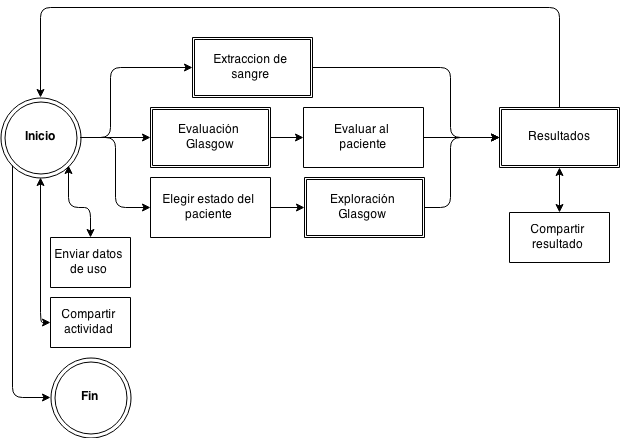
\includegraphics[scale=0.5]{propuesta/grafo_escenas.png}
\caption{Navegación entre escenarios y pantallas. Los escenarios son los
    rectángulos con un borde de dos rayas, y las pantallas tienen un borde con una
    sola raya. Los estados inicial y final se muestran como círculos, notar que
    el estado inicial es además del punto de entrada, un escenario.}
\label{fig:grafo_estados}
\end{figure}

La solución inicia con un escenario denominado \emph{Inicio}, en el cual se
permite al usuario observar los detalles del entorno simulado a la vez que
muestra las opciones que permiten iniciar las diferentes prácticas, compartir
su actividad, enviar los datos de utilización y finalmente salir de la
simulación.

Si el usuario selecciona en el \emph{inicio} la opción \emph{Extracción de
    sangre}, se inicia el escenario denominado \emph{Extracción de sangre}, en
el cual el usuario puede realizar el procedimiento de extracción de sangre, si
el usuario selecciona la opción \emph{Fin}, la simulación termina y se dirige 
al escenario \emph{Pantalla de resultados}.

Al seleccionar la opción \emph{Evaluación Glasgow}, se inicia el escenario
denominado \emph{Glasgow}, donde el usuario debe evaluar a un paciente en el
centro del escenario, si el usuario presiona la opción \emph{Fin} se inicia la
pantalla denominada \emph{Evaluar al paciente}, donde el usuario diagnostica el
estado del paciente, y finalmente al presionar el botón \emph{Fin}, la
simulación finaliza y se inicia el escenario \emph{Pantalla de resultados}.

La opción \emph{Exploración Glasgow} es similar, la diferencia es que antes de
iniciar el escenario \emph{Glasgow}, aparece la pantalla \emph{Elegir estado de
    paciente}, en el cual el usuario selecciona un estado para que el paciente
actué de acuerdo al mismo, luego se inicia la escena \emph{Glasgow} y si el
usuario presiona el botón \emph{Fin}, se inicia el escenario \emph{Pantalla de
    resultados}.

La pantalla de resultados muestra la información acerca de las acciones que
realizó el usuario, proveyendo información a modo de retroalimentación, en esta
pantalla el usuario puede compartir sus resultados por las redes sociales,
reiniciar el escenario y finalmente, puede volver a la \emph{Pantalla de
    inicio}.

A continuación, se describen todos los escenarios, primeramente se da una 
descripción general de los escenarios y se procede a explicar los detalles 
de los mismos, incluyendo las entidades, eventos y acciones que pueden ser realizados 
en el mismo.

\subsection{Inicio}

La solución se inicia con un escenario que esta inspirado en el laboratorio de
enfermería del \Gls{iab}, es la primera experiencia que tiene un
usuario al utilizar la misma, sirve como un menú principal, desde
este punto todas las opciones son accesibles para el usuario, este escenario es
denominado~\emph{Inicio}.

La primera vez que se inicia la solución, se muestra una pequeña ventana
solicitando el número de teléfono del usuario, se utiliza esta información como un
identificador del usuario para así poder asociar la información del mismo con un
alumno en particular.

\subsubsection{Descripción del entorno}
\label{sec:inicio_descripcion}

La escena mostrada como pantalla de inicio de la aplicación muestra como fondo
la sala de un hospital con los elementos típicos de estos lugares, esta es la
que se utiliza como escenografía principal en las escenas de los procedimientos.
Además de este fondo, se muestran varias opciones en forma de botones que serán
descriptas a continuación y un mensaje en donde se recomienda al usuario el uso
de auriculares.

\begin{figure}[H] 
\centering 
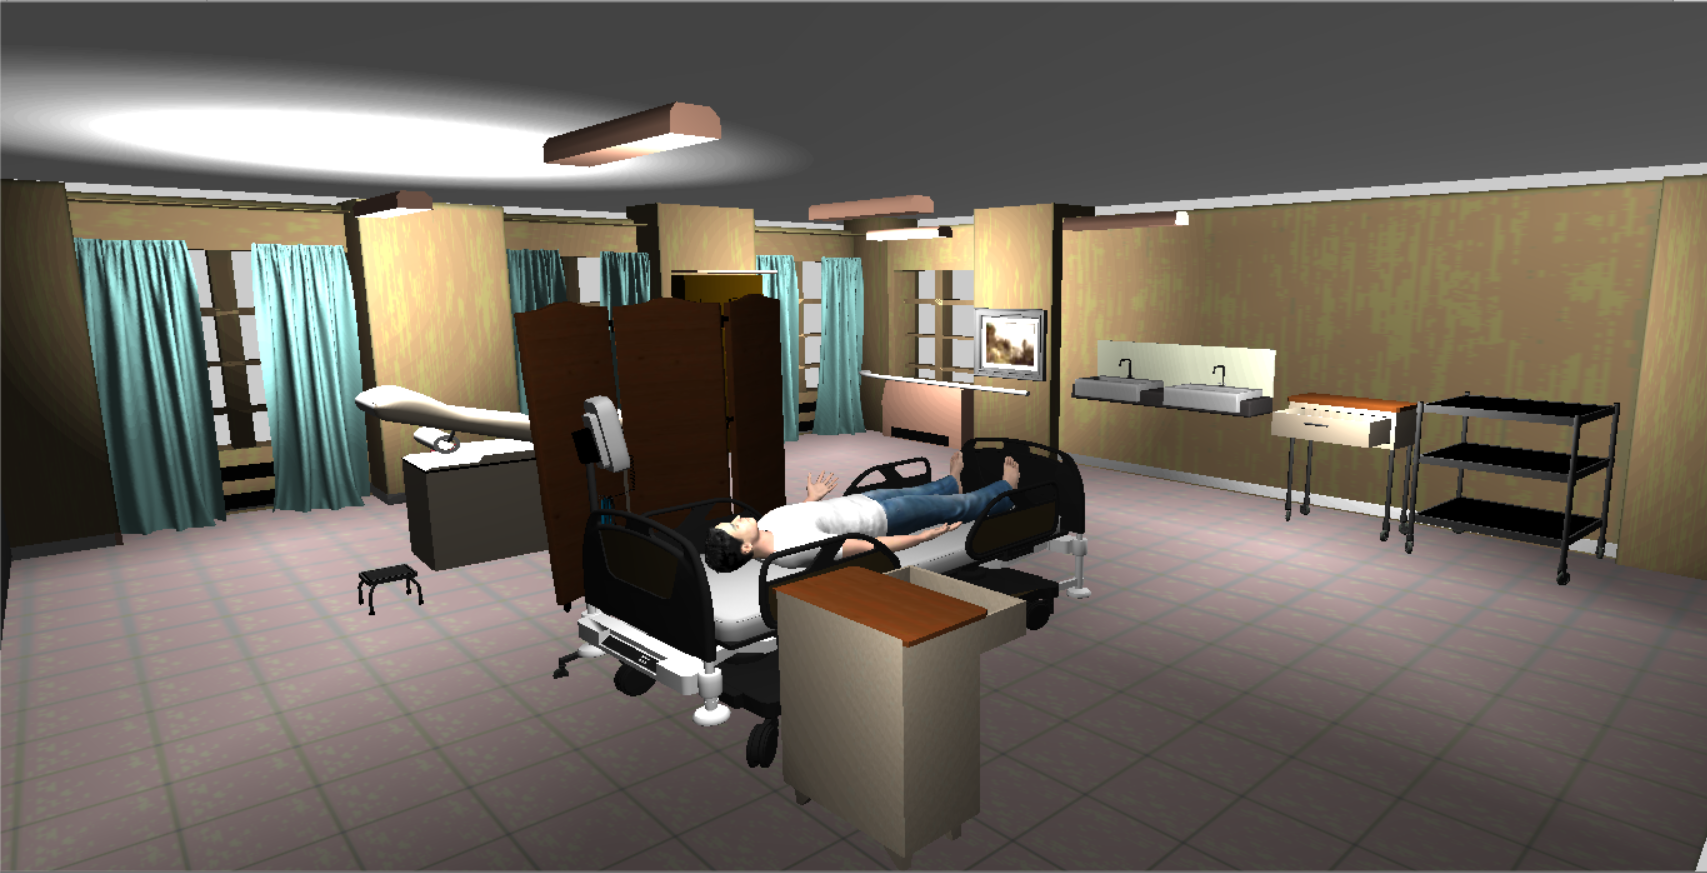
\includegraphics[scale=0.2]{propuesta/sala.jpg}
\caption{Edificio y decoración inspirados en los laboratorios de enfermería del
    \Gls{iab}, este edificio se utiliza para los diferentes escenarios}
\label{fig:sala_perspectiva}
\end{figure}

Se observa en la figura~\ref{fig:sala_perspectiva} la decoración utilizada en
el escenario \emph{Inicio}, mientras se muestran las opciones, se ejecuta una
animación que recorre el escenario mostrando los detalles importantes, como la
camilla, el lector de estadísticas vitales, y demás elementos del escenario.

\subsubsection{Opciones}

Las opciones disponibles en la pantalla de inicio son presentadas en forma de
botones los cuales tienen una breve descripción que identifica la función que
cumplen. 

\begin{itemize}
\item Botón \enquote{Enviar Progreso}: esta función envía toda la información
    acerca de la actividad que el usuario realizó en la aplicación a un servidor
    \emph{backend} que se encarga de almacenar estos datos.
\item Botón \enquote{Salir de la simulación}: esta función permite salir de la
    aplicación.
\item Botón \enquote{Facebook}: esta función permite al usuario ingresar a su
    cuenta de Facebook.
\item Botón \enquote{Extracción de sangre}: esta función permite ingresar a la
    escena correspondiente al procedimiento de extracción de muestras de sangre
    permitiendo al usuario jugar una nueva partida.
\item Botón \enquote{Explorar Glasgow}: esta función permite ingresar a la
    escena correspondiente al procedimiento para explorar las reacción de un
    paciente con un diagnóstico específico de la escala de Glasgow permitiendo
    al usuario jugar una nueva partida, el diagnóstico se selecciona una vez
    presionado este botón a través de la ventana de~\emph{Elegir estado del
        paciente}.
\item Botón \enquote{Evaluar Glasgow}: esta función permite ingresar a la escena
    correspondiente al procedimiento para la valoración y diagnóstico de la
    escala de Glasgow para un paciente con estado aleatorio permitiendo al
    usuario jugar una nueva partida.
\end{itemize}


\subsection{Extracción de muestras de sangre}

A continuación se detallan cada una de las opciones y formas disponibles de
interactuar con la escena del procedimiento de extracción de muestras de sangre.

Los detalles a continuación toman en cuenta las hipótesis definidas
en~\ref{sec:hemocultivo_hipotesis}. 

\subsubsection{Descripción del entorno}

Al seleccionar el procedimiento de extracción de sangre en la pantalla de inicio 
la aplicación inmediatamente muestra la escena del procedimiento, se muestra una 
sala de hospital igual a la de la pantalla de inicio pero con un paciente en una 
de las camas, a este paciente es a quien se le realizará el procedimiento.

La posición inicial de la cámara se ubica en un ángulo en donde se puedan ver 
bien los brazos del paciente para facilitar al usuario la realización del 
procedimiento.


\subsubsection{Entidades}

En la extracción de sangre existen dos entidades principales, el \emph{paciente}
y el \emph{usuario}, cada entidad mantiene un estado independiente de la otra
entidad.

El \emph{paciente} es una entidad con estado complejo, el cual es constantemente
modificado por las acciones del usuario, en resumen, la información que contiene
el paciente es:

\begin{itemize}
    \item \textbf{Jeringas}: un paciente puede tener cero o más jeringas en
        cualquier momento, no se limita la cantidad de jeringas que puede
        insertar el usuario.
    \item \textbf{Manos}: almacena el estado de las manos, el paciente reacciona
        ante peticiones del usuario, puede abrir o cerrar cualquier mano en
        cualquier momento.
    \item \textbf{Torniquetes}: es el conjunto de torniquetes que tiene
        actualmente el paciente, notar que los torniquetes pueden ser colocados
        en cualquier parte del brazo, pero existen lugares \enquote{correctos} y
        lugares \enquote{incorrectos}, la diferencia consiste en la distancia a
        los puntos de extracción, estos lugares están predefinidos.
    \item \textbf{Zonas esterilizadas}: son aquellas áreas del cuerpo que el
        usuario esterilizó, no existe un límite para las zonas esterilizadas.
        Una vez que una jeringa es extraída, una zona esterilizada pasa a estar
        contaminada y a la espera de que el usuario la presione.
    \item \textbf{Zonas presionadas}: son aquellas zonas que, una vez
        contaminadas por la extracción de una jeringa, han sido presionadas por
        el usuario.
    \item \textbf{Contaminado}: define si alguna acción realizada por el usuario
        provocó que el paciente se contamine, existen varias cadenas de eventos
        que pueden hacer que esto ocurra:
        \begin{itemize}
            \item Inyección de una jeringa cuando existe otra inyectada.
            \item Inyección en un lugar inadecuado.
            \item Inyección en un lugar no esterilizado.
            \item Inyección en un brazo cuya mano este abierta.
            \item Inyección fuera del alcance de los torniquetes actuales.
            \item Interacción con el paciente sin que el enfermero tenga la mano
                estéril.
        \end{itemize}
        Es importante notar que este estado no es afectado directamente por una
        acción del usuario, sino por la consecuencia de una acción.
\end{itemize}

El \emph{usuario o enfermero} mantiene un estado en todo momento del cual
dependen sus acciones, por ejemplo, si la mano del enfermero no está
esterilizada, cualquier interacción con el paciente provocará que se
contamine.

\begin{itemize}
    \item \textbf{Manos}: almacena la información acerca de la esterilidad de
        las manos.
    \item \textbf{Guantes, gorro, bata y tapaboca}: almacenan la información
        acerca de los equipamientos que tiene el usuario en un momento dado.
    \item \textbf{Elemento actual}: es el elemento que está activo en
        cualquier momento, un elemento es una herramienta de la vida real,
        como por ejemplo un torniquete, una gaza.
\end{itemize}

\subsubsection{Acciones}

Las acciones que puede realizar el usuario se clasifican en tres, los
\emph{comandos de voz} que simulan una conversación entre el paciente y
enfermero, \emph{las opciones}, que engloban las acciones que puede realizar un
enfermero en cuanto a bioseguridad, y \emph{los elementos} que son las
herramientas que puede utilizar el enfermero durante el procedimiento.

\paragraph{Comando de voz}

Para representar la interacción del usuario con el paciente usando la voz se
implementó un menú que es activado y mostrado en pantalla cuando el usuario
habla, este menú muestra una serie de órdenes que el usuario le diría al
paciente normalmente. Las opciones de menú se detallan a continuación:

\begin{itemize}
    \item \textbf{Explicar procedimiento}: Permite que el usuario explique el
        procedimiento que se va a realizar al paciente. 
\item \textbf{Abrir la mano izquierda}: esta función le indica al paciente que
    abra su mano izquierda, como resultado el paciente realiza esta acción.
\item \textbf{Cerrar la mano izquierda}: esta función le indica al paciente que
    cierre su mano izquierda, como resultado el paciente realiza esta acción.
\item \textbf{Abrir la mano derecha}: esta función le indica al paciente que
    abra su mano derecha, como resultado el paciente realiza esta acción.
\item \textbf{Cerrar la mano derecha}: esta función le indica al paciente que
    cierre su mano derecha, como resultado el paciente realiza esta acción.
\end{itemize}

\begin{figure}[H]
\centering

\includegraphics[scale=0.5]{propuesta/hemocultivo_comando_voz.jpg}
\caption{Opciones mostradas al detectar sonido en la escena de extracción
    de sangre.}
\label{fig:hemocultivo_voz_gui}
\end{figure}

En la figura~\ref{fig:hemocultivo_voz_gui} se observan las opciones anteriormente
descritas, este menú aparece inmediatamente después de que el sistema detecte
que el usuario este hablando.

\paragraph{Opciones}

Las \emph{Opciones} son aquellas acciones que puede realizar el usuario y afectan
únicamente al paciente. Representan a los aspectos de bioseguridad, es decir,
acciones como lavarse las manos, calzarse guantes, gorro, bata y tapaboca.

Estas opciones afectan al estado de la entidad \emph{enfermero}.

\paragraph{Elementos}

Los \emph{Elementos} representan las herramientas que utiliza un enfermero
durante el procedimiento, un solo elemento puede ser utilizado en cualquier
momento.


\begin{figure}[H]
\centering
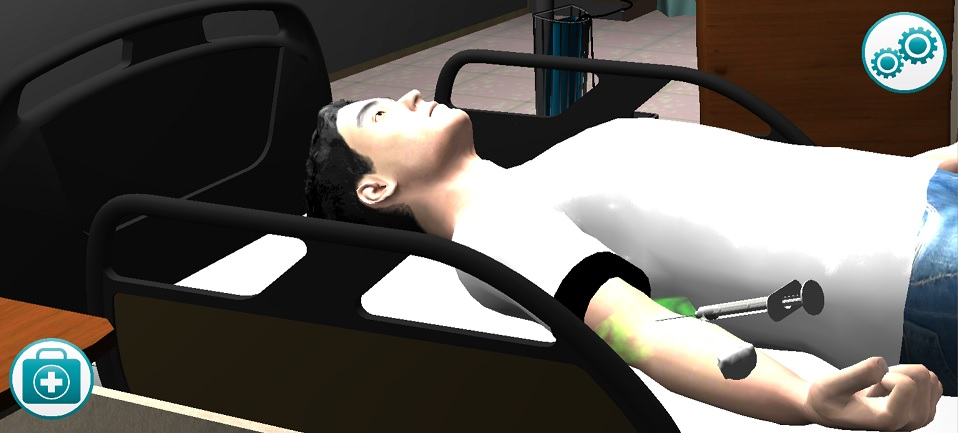
\includegraphics[scale=0.5]{propuesta/hemocultivo_elementos.jpg}
\caption{Interfaz con los elementos en el paciente, se observa el torniquete (es
    un toro negro), la jeringa, una zona esterilizada (el área cerca del
    torniquete) y un algodón para punzar (Cerca de la muñeca, es una figura
    blanca), todo en el brazo derecho.}
\label{fig:hemocultivo_elementos}
\end{figure}

Los elementos, que podemos observar en la
figura~\ref{fig:hemocultivo_elementos}, son:

\begin{itemize}
\item \textbf{Torniquete}: es el primer elemento que se debe usar, para utilizarlo
    , el mismo se activa al presionar una parte del brazo del paciente,
    en ese momento, el torniquete aparece en el brazo del paciente, para
    extraerlo, se debe presionar el torniquete y elegir la opción extraer. En la
    figura~\ref{fig:hemocultivo_elementos} se observa al torniquete como un toro
    negro alrededor del brazo izquierdo.

\item \textbf{Esterilizador}: es un elemento que se utiliza para realizar la
    higienización del punto de punción, para utilizarlo se debe presionar
    cualquier parte del brazo del paciente, a continuación aparece una gaza, la
    cual debe ser agitada con un dedo durante un segundo para que se cree una
    zona estéril, la zona estéril creada, es visible a través de una cápsula
     transparente de color verde.

\item \textbf{Jeringa}: Es el elemento utilizado para realizar la extracción, su
    utilización es similar a la del \emph{Torniquete}, solo que además de la
    opción de extracción tiene dos opciones adicionales.

    A través de un menú contextual, se ofrece la posibilidad de realizar un
    acercamiento, como se observa en la
    figura~\ref{fig:hemocultivo_jeringa_zoom}, en la vista ampliada, se puede
    realizar la extracción de sangre utilizando dos dedos, con el primero se
    presiona el tambor y con el segundo dedo se extrae el émbolo\footnote{El
        tambor es la parte de la jeringa que almacena el fluido, mientras que el
        émbolo es la parte que se utiliza para presionar o succionar el fluido}.
    
\item \textbf{Algodón}: El algodón se utiliza para presionar una zona que
    recientemente fue punzada, para utilizar este elemento, basta con presionar
    el brazo del paciente durante un segundo.

\end{itemize}


\begin{figure}
\centering
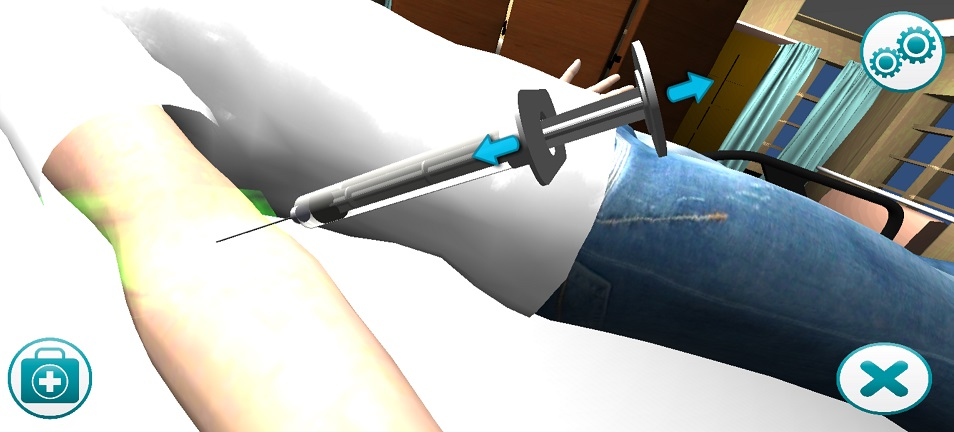
\includegraphics[scale=0.5]{propuesta/hemocultivo_jeringa_ampliada.jpg}
\caption{Vista de la jeringa ampliada, facilitando la extracción de sangre. Se
    agregan flechas azules para facilitar la comprensión del cómo se extrae
    sangre.}
\label{fig:hemocultivo_jeringa_zoom}
\end{figure}



\subsubsection{Reglas para la evaluación durante la ejecución}

%La reglas del procedimiento de extracción de sangre fueron definidas de acuerdo
%a los pasos requeridos según el protocolo del procedimiento y al orden en el que
%son requeridos. Es decir, cada paso del protocolo tiene asociado una regla
%dentro del motor que lo representa y las condiciones asociadas a cada regla
%están determinadas por el orden en que deben realizarse dentro del protocolo.

%Cada regla tiene una o mas condiciones que deben ser cumplidas para que un paso
%del protocolo realizado se considere correcto.

Las reglas definidas dentro de la extracción de sangre definen las acciones
que se deben llevar a cabo para completar el procedimiento, es necesario que
todas las reglas sean cumplidas para obtener un puntaje perfecto.

Cada regla contiene información acerca del estado del progreso del alumno en un
paso en particular, estas reglas pueden tener como dependencias a otras reglas,
es decir, una regla sólo se puede cumplir si una regla anterior se cumple, este
es el caso de las reglas que definen la extracción de un torniquete, la cual
depende de la regla que define la colocación del torniquete.  

Las reglas definen el mecanismo que se utiliza para proveer una retroalimentación
al usuario una vez finalizada la partida, pues la regla almacena información 
acerca del progreso del usuario en cada paso.

A continuación se da una breve descripción de las reglas utilizadas y sus
diversos estados.

\begin{itemize}
\item \textbf{Explicar procedimiento}: define cuando el usuario ha explicado el
    procedimiento, debe ser la primera regla que se cumple, existiendo dos
    estados que no cumplen la condición, cuando no es la primera regla que se
    cumple y cuando el usuario no realizó la acción.

\item \textbf{Higienización de manos}: define sí las manos del enfemero están
    limpias, existen dos estados para esta regla, cuando se lavó las manos y
    cuando no realizó esta acción. Es importante notar que de esta regla
    dependen varias reglas posteriores, es decir, si esta regla no se cumple,
    las reglas de bioseguridad no pueden ser cumplidas.

\item \textbf{Calzar guantes}: este paso es inmediatamente posterior a la
    higienización de las manos, y como este, varias reglas dependen del momento
    en el que se calcen los guantes. Si el paciente se calza los guantes, la
    única forma de equivocarse en este paso es que las manos estén sucias.

\item \textbf{Gorro, bata y tapaboca}: estos tres pasos son similares, pues
    tienen las mismas dependencias y el orden en el que se cumplan no está
    definido, las posibilidades con este paso son:
    \begin{itemize}
    \item Incompleto: si el usuario no se puso el gorro, bata o tapaboca en
        ningún momento de la práctica.
    \item Manos sucias: si la regla \emph{Higienización de manos} no se cumple
        cuando el usuario se vista con el gorro, bata o tapaboca.
    \item Sin guantes: si la regla \emph{Calzar guantes} no se cumple al momento
        de ponerse el gorro, tapaboca o bata. 
    \end{itemize}
    
\item \textbf{Colocar torniquete}: este paso debe ser realizado una vez que el
    usuario tenga el guante calzado, el torniquete puede ser colocado en
    cualquier parte del brazo, pero depende del lugar de punción de la jeringa.
    Así, existen dos casos donde esta regla falla, cuando no se coloca el
    torniquete en ningún lugar, y cuando el torniquete se coloca en un lugar
    inadecuado. Es importante notar que esta regla se activa cuando se realiza
    la punción de la jeringa.

\item \textbf{Cerrar manos}: debe ocurrir después de que se explique el
    procedimiento y antes de que se inserte la jeringa, además deberá ser la
    mano correspondiente al lugar donde se inyectó la jeringa. Así, existen dos
    formas de no realizar correctamente este paso, que la punción haya ocurrido en otro brazo, o
    que la punción no se realizó. Es importante notar que esta regla no se activa
    cuando el usuario solicita al paciente que cierre su mano, sino cuando la
    jeringa es insertada, esto es así pues es importante el estado de la mano
    cuando el usuario realiza la punción.

\item \textbf{Esterilizar zona}: El usuario puede esterilizar varias zonas, pero
    la única zona que activa esta regla, es aquella donde se realizó la punción.
    Así esta regla tiene dos posibles formas de proveer retroalimentación en
    caso de que no se cumpla, que no se esterilizó ningún lugar del cuerpo, o
    que el lugar esterilizado no sea el lugar de punción.

\item \textbf{Realizar punción}: Existen dos casos de error, si el usuario
    inserta la jeringa en un lugar incorrecto (los lugares correctos se definen
    en~\ref{sec:hemocultivo_hipotesis}), y si el usuario no realiza la punción.

\item \textbf{Retirar Torniquete}: esta regla es dependiente de la regla
    \emph{Colocar Torniquete}, y de qué torniquete se retira. Existiendo dos
    casos de error, el usuario retira un torniquete que no activó la regla
    \emph{Colocar Torniquete} (indicando que este es el torniquete correcto), y
    que no se retire ningún torniquete.

\item \textbf{Abrir mano}: una vez realizada la punción, y retirado el torniquete,
    se debe solicitar al paciente que abra sus manos, así, es dependiente de la
    regla \emph{Realizar punción}, y tiene tres casos de error, que la punción
    no se haya realizado, que la mano no se haya cerrado antes, y que la mano
    que se abra no corresponda con la mano que se cerró.

\item \textbf{Extraer Sangre}: depende únicamente de si la jeringa con la cual
    se extrae sangre es la correcta, así hay dos posibles casos de error, que
    la sangre no se haya extraído, y que la regla \emph{Realizar punción} no se
    cumpla.

\item \textbf{Retirar Jeringa}: se controla que la jeringa que se extraiga sea
    la jeringa que cumplió el paso \emph{Realizar punción}, así, existen dos
    casos de error, que la jeringa no hay sido extraída y que se extrajo sangre
    de una jeringa incorrecta.

\item \textbf{Presionar zona de punción}: debe realizarse inmediatamente después
    de \emph{Retirar Jeringa}, y tiene dos casos de error, que la jeringa no
    haya sido extraída, y que la zona presionada no corresponda con la zona de
    punción.

\item \textbf{Quitar bata, gorro y tapaboca}: depende de la regla \emph{Bata,
        gorro y tapaboca}, y de que la jeringa haya sido extraída, si el
    enfermero se extrae la bata, gorro o tapaboca antes de retirar la jeringa, se
    produce un error. Otro caso para que esta regla no se cumpla es que la regla
    \emph{Bata, gorro y tapaboca} no se cumpla.

\item \textbf{Descalzar guantes}: depende de que las reglas \emph{Calzar
        Guantes} y \emph{Retirar jeringa}, así existen dos posibles casos de
    error, que el usuario no se calce los guantes, o que la jeringa no haya sido
    extraída.

\item \textbf{Limpiar manos}: Como paso final, se debe proceder a realizar una
    higienización de manos, este debe ser el paso final, y tiene como
    prerrequisito que todas las reglas anteriores hayan sido lanzadas.

\end{itemize}

\paragraph{Retroalimentación y puntuación final}
\label{sec:puntuacion_hemocultivo}

Cada regla tiene asociado un peso, de acuerdo a la dificultad de realizar el
paso, este peso es utilizado al final de la partida para darle una puntuación al
usuario acerca de su rendimiento en la partida.

Además, un regla puede quedar en uno de diferentes estados al final de la
partida como se mostró anteriormente, cada uno de esos estados posee un
significado en el contexto del procedimiento y por lo tanto tienen información
asociada para que al final de la partida se muestre una retroalimentación
correcta al usuario por paso realizado o no.

\subsubsection{Registro de actividad}

Cada acción que realiza el usuario dentro de la simulación provoca un evento, y
estos eventos son registrados de manera transparente para el usuario.

Existen otros tipos de eventos que no son generados por acciones, por ejemplo,
cuando la simulación termina, el motor de reglas lanza un evento por regla,
indicando su estado.

Un subconjunto de todos los eventos, son registrados en un archivo de texto en
formato \Gls{json}, el mismo es posteriormente enviado a un servidor que
almacena la información de todos los usuarios.

Los eventos registrados, son aquellos que involucran a las opciones, elementos,
utilización de la jeringa, torniquete, higienización, y como un caso especial,
todas las reglas también son registradas (independientemente de si son
satisfactorias o no).

La información que se almacena permite reproducir exactamente todo el desarrollo
de la simulación, con excepción de los movimientos de la cámara. De esta manera,
los datos recabados permiten saber en que tareas los usuarios se encontraron con
un mayor número de inconvenientes.

\subsubsection{Interfaz del usuario}

La interfaz principal de este escenario posee dos menús, uno a cada lado de la
pantalla, las opciones son representadas como botones que poseen una imagen
intuitiva que representa la función que realizan. 

\begin{figure}
\centering

\includegraphics[scale=0.5]{propuesta/hemocultivo_gui.jpg}
\caption{Vista de la interfaz principal del escenario \emph{Extracción de
        sangre}, con todas las opciones desplegadas.}
\label{fig:hemocultivo_gui}
\end{figure}


En la figura~\ref{fig:hemocultivo_gui} se observa la interfaz, se muestra en el
centro al paciente, y las diferentes opciones que tiene el usuario para
interactuar con el paciente y consigo mismo como enfermero.

Existen dos opciones principales dentro de la interfaz, en la parte superior
derecha se encuentra el menú \emph{Opciones} y en la parte superior izquierda, el menú
\emph{Elementos}.

Al presionar el menú \emph{Opciones} aparecen las distintas
acciones que puede realizar el usuario en cuanto a aspectos de bioseguridad, el 
lavado de manos es idempotente, es decir no importa cuantas veces se presione, el 
resultado será el mismo, en cambio los demás botones (bata, guante, tapaboca y gorro)
representan la acción de calzar/descalzar, es decir, la primera vez que se presiona
la opción bata, el estado del enfermero cambia a \emph{Con Bata}, si se presiona una
segunda vez, el estado cambia a \emph{Sin Bata}.

En el menú \emph{Elementos} se despliegan opciones que representan a lo elementos que se
utilizan para realizar el procedimiento, una vez presionado un elemento queda
seleccionado (simulando que es la herramienta que el enfermero tiene en la mano
en ese momento), sólo un elemento puede ser seleccionado a la vez. Si el mismo
botón se vuelve a presionar inmediatamente después de haber sido presionado, el
elemento se des-selecciona (simulando que el enfermero dejó la herramienta).

Adicionalmente, existen dos indicadores del estado del paciente, en la parte
inferior derecha, denominados \emph{Indicadores de bioseguridad}, se muestran
iconos representando los elementos que tiene actualmente el enfermero, estos
incluyen los gorros, bata y tapaboca. El elemento que actualmente esta
seleccionado se muestra en la parte superior izquierda de la pantalla, a
diferencia de los indicadores de bioseguridad, se muestra un único icono a la vez.

Para la utilización de los elementos, existe un menú contextual\footnote{Un menú
    que se despliega al presionar un elemento, es contextual pues varía de
    acuerdo al elemento seleccionado.}, que lista las opciones disponibles por
elemento, como se observa en la figura~\ref{fig:hemocultivo_torniquete_cm}.

\begin{figure}
\centering
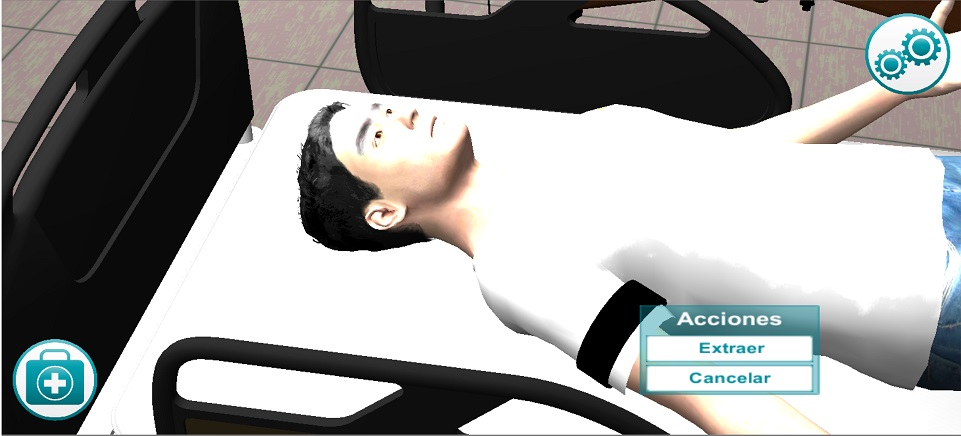
\includegraphics[scale=0.5]{propuesta/hemocultivo_contextual.jpg}
\caption{Menú contextual del elemento torniquete.}
\label{fig:hemocultivo_torniquete_cm}
\end{figure}

\subsection{Valoración de la escala de Glasgow}


La escena  \emph{Valoración de la escala de Glasgow} busca simular el
comportamiento de un paciente con daño cerebral, por ello se presenta en dos
modos distintos, en la primera, el usuario no conoce el estado del paciente,
este modo se conoce como \emph{Evaluar Glasgow}, y en su segundo modo, el
usuario elige el estado del paciente antes de iniciar la escena, esto modo
se conoce como \emph{Exploración Glasgow}. 

La reducida cantidad de diferencias entre ambos modos de la práctica permiten
que ambas sean descritas en esta sección, las características explicadas son
comunes para ambas, salvo que se especifique lo contrario.

En el modo \emph{Exploración Glasgow}, antes de iniciar la práctica, se le
permite al usuario seleccionar el estado del paciente mediante una interfaz, en
cambio, en el modo \emph{Evaluar Glasgow}, el estado del paciente no se conoce
de antemano y será responsabilidad del usuario determinarlo.

La escena se inicia mostrando un paciente acostado en una camilla, de manera
similar a la escena \emph{Extracción de sangre}, la principal diferencia es que
el paciente no se encuentra en ninguna posición en particular, simplemente esta
acostado en la camilla.

Existe una pantalla particular dentro de esta escena, conocida como
\emph{Pantalla de Diagnóstico}, esta pantalla, permite al usuario ingresar su
diagnóstico del paciente, contiene cuatro preguntas básicas, la valoración
motora, verbal, ocular y general de acuerdo a lo definido en~\ref{sec:glasgow} y
a las hipótesis definidas en~\ref{sec:glasgow_hipotesis}.

\emph{Exploración Glasgow}.

\subsubsection{Entidades}

Al igual que en \emph{Extracción de sangre}, existen dos entidades principales,
pero en esta escena, el enfermero no almacena información alguna, y el
paciente sólo almacena su estado, que se define al inicio. De esta forma, las
entidades no se modifican en ningún momento.

La información almacenada por la entidad paciente es su estado motor, verbal y
ocular, el cual es un conjunto de números, cuyos posibles valores se definen en
en~\ref{sec:glasgow_protocolo}, la definición de estos números varían de acuerdo
al tipo de la escena:

\begin{itemize}
    \item \textbf{Exploración}: la escena de exploración se inicia con la
        \emph{Pantalla de diagnóstico}, donde el usuario selecciona el estado
        del paciente que desea, este estado se mantendrá constante durante toda
        la escena.
    \item \textbf{Evaluación}: al inicio se crean tres números de manera
        aleatoria, el algoritmo que crea estos valores, lo hace de tal manera
        que el estado del paciente es consistente, por ejemplo, el paciente
        nunca tendrá un estado verbal \enquote{Orientado} (valor 5 en la escala)
        y un estado ocular \enquote{Ausente} (valor 1 en la escala), pues esto
        no tendría sentido, si no puede abrir los ojos (estado
        \enquote{ausente}), no puede saber donde esta (estado
        \enquote{orientado}).
\end{itemize}

Aunque el estado de las entidades no se modifique, esto no significa que no
puedan realizar acciones entre ellas, sino que estas acciones y los eventos
generados no alteran el estado de las entidades.

\subsubsection{Acciones} 

Las acciones se clasifican en dos tipos, los \enquote{comandos de voz} y las
\enquote{opciones a través de menú contextual}. 

\paragraph{Menú Contextual}

Las opciones a través del menú contextual se relacionan a acciones que puede
realizar el enfermero sobre una parte particular del cuerpo del paciente, en las
extremidades, el menú despliega una sola opción, la cual es \emph{Pinchar}, que
provoca que el enfermero realice un estímulo doloroso al paciente, el
paciente reacciona ante este estímulo dependiendo de su valoración motora y
ocular. 

\begin{itemize}
    \item Si el estado ocular del paciente es \enquote{Al dolor}, el paciente
        abrirá los ojos inmediatamente después de que se presione la opción. 
    \item  La respuesta motora varía de acuerdo a su estado, si el mismo es
        \enquote{Localiza}, el paciente mueve sus manos hasta el origen del
        dolor, si el estado es \enquote{Retira}, moverá la extremidad que
        sufrió el estímulo lejos de su posición inicial, si es
        \enquote{Flexión anormal}, el paciente reaccionará comprimiendo el
        cuerpo, indistintamente de la ubicación del estímulo doloroso, y si el
        estado es \enquote{Extiende}, el paciente extenderá el cuerpo.
\end{itemize}

\paragraph{Comandos de voz}

Las opciones disponibles a través de los comandos de voz, simulan una
interacción verbal entre el enfermero y el paciente, y se agrupan en tres
tipos, verbales, oculares y motoras.

Las preguntas y posibles respuestas de tipo \emph{verbal}, se pueden ver en la
tabla~\ref{tab:glasgow_opciones_respuesta}. 

\begin{table}[H]
\centering
\begin{tabulary}{1.2\textwidth}{LCCCCC}
\toprule
\textbf{Pregunta} & \textbf{Orientado} & \textbf{Confusa} & \textbf{Palabras
    inapropiadas} & \textbf{Palabras incomprensibles} & \textbf{Ausente} \\
\midrule
¿Qué día es? & El día de la semana actual & Cualquier día de la semana menos el
correcto & La respuesta a otra pregunta en estado orientado & Gritos, gruñidos y
quejidos & No emite sonido \\
¿Cuál es su nombre? & \emph{Carlos Benitez} & Respuesta coherente sin mencionar
su nombre & Respuesta a otra pregunta en estado orientado & Gritos, gruñidos y
quejidos & No emite sonido \\
¿Donde se encuentra? & \emph{En una cama de hospital} & \emph{En mi dormitorio} &
Respuesta a otra pregunta en estado orientado & Gritos, gruñidos y quejidos & No
emite sonido \\
\bottomrule
\end{tabulary}
\caption{Posibles respuestas de acuerdo al estado verbal del paciente.}
\label{tab:glasgow_opciones_respuesta}
\end{table}

Las opciones del menú por comandos de voz del tipo \emph{motor}, son cuatro: 

\begin{itemize*}
    \item Mueva el brazo
    \item Mueva la pierna
    \item Mueva la mano
    \item Mueva la cabeza
\end{itemize*}

A diferencia de las opciones verbales, estas no tienen una respuesta sonora, en
cambio, si el estado motor es \enquote{Obedece},el paciente reacciona moviendo
una extremidad, en caso contrario, el paciente no realiza acción alguna.

Finalmente, existe una opción \emph{ocular}, la cual es \enquote{Abra sus ojos por
favor}, la cual no tiene una respuesta sonora, y sólo si el paciente tiene un
estado ocular \enquote{Al hablar} abre los ojos, en caso contrario, no realiza
acción alguna.

\subsubsection{Pantalla de diagnóstico}

Una vez que el usuario decida que está listo para dar un diagnóstico, procede a
finalizar la escena, en ese momento se presenta una pantalla donde el mismo
puede diagnosticar al paciente, como se observa en la
figura~\ref{fig:glasgow_gui_resultados}.

Las opciones presentadas al usuario son cuatro, puntuación verbal, ocular,
motora y un diagnóstico del estado de conciencia del paciente. Estos valores
se describen en~\ref{sec:glasgow_protocolo}.

\begin{figure}[H]
\centering
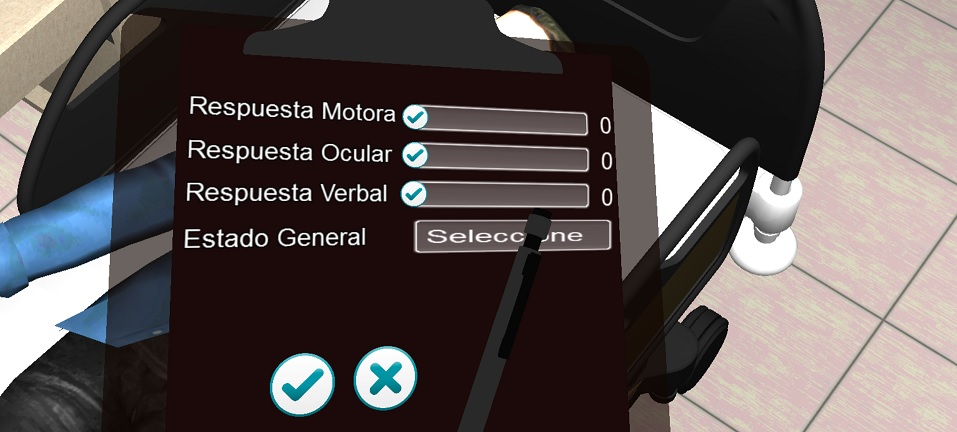
\includegraphics[scale=0.5]{propuesta/glasgow_diagnostico.jpg}
\caption{Vista de la \emph{Pantalla de diagnóstico}, donde el usuario puede
    asignar una puntuación a cada aspecto analizado del paciente.}
\label{fig:glasgow_gui_resultados}
\end{figure}

En el modo \emph{Evaluación Glasgow}, esta misma pantalla se utiliza la inicio
de la escena para que el usuario pueda seleccionar el estado deseado del
paciente.

La única diferencia que existe entre la \emph{Pantalla de diagnóstico} entre la
exploración y la evaluación, es que en la evaluación, los posibles valores para
cada aspecto a diagnosticar van de $0$ a $8$, y en la exploración, son los
valores mínimos y máximos válidos\footnote{Los valores máximos se definen
    en~\ref{sec:glasgow_protocolo} y son $4$ (ocular), $5$ (verbal) y $6$
    (motora)}.

\subsubsection{Valoración}
\label{sec:puntuacion_glasgow}

Para la evaluación del rendimiento del usuario al momento de llevar a cabo el
procedimiento de valoración de la escala de Glasgow se tuvo un enfoque
completamente diferente al del procedimiento de extracción de sangre debido a la
naturaleza propia del procedimiento. 

Como se explicó anteriormente, el paciente puede estar en ciertos estados
específicos dentro de la escala, y además dentro de cada estado reacciona de una
forma en particular, por lo tanto, al inicio de la partida un componente interno
de la aplicación selecciona de forma aleatoria un estado para el paciente, de
forma tal que cada vez que una partida sea jugada no se repitan los estados de
forma seguida.

El estado aleatorio del paciente es guardado en una variable que no es
modificada hasta que se reinicie la partida. Al final de la partida, la
aplicación pide al usuario que valore el estado del paciente que le fue
presentado, una vez que el usuario confirme su respuesta la aplicación la
compara con el estado guardado y de esta forma puede informar al usuario acerca
de su rendimiento en el diagnóstico.

Además, cada posible respuesta dada por el usuario contiene información
relacionada al contexto del procedimiento y a la situación actual presentada, la
cual, es utilizada como retroalimentación al final de la partida. La puntuación
final depende de la cantidad de valoraciones correctas dadas por el usuario
para la respuesta verbal, motora, ocular y nivel de gravedad del paciente.

\subsubsection{Registro de actividad}

Al igual que en la escena de \emph{Extracción de sangre}, las acciones del usuario
son registradas en un archivo con formato \Gls{json} y enviadas a un servidor
que almacena la información acerca de todos los usuarios.

Se almacena además, el diagnóstico del usuario, la puntuación del mismo y el
estado inicial del paciente, así como el modo de la escena (evaluación o
exploración).

\subsubsection{Interfaz de usuario}

La interfaz de usuario, como se observa en la figura~\ref{fig:glasgow_gui}, es
muy sencilla, se compone de solo una opción permanente, la cual permite al
usuario finalizar la escena y mostrar la \emph{Pantalla de diagnóstico}. Se
observan además, las opciones que se despliegan cuando la solución detecta que el
usuario emite palabras, conocidas como \emph{Comandos de Voz}, que permiten al
mismo interactuar con el paciente.

\begin{figure}[H]
\centering
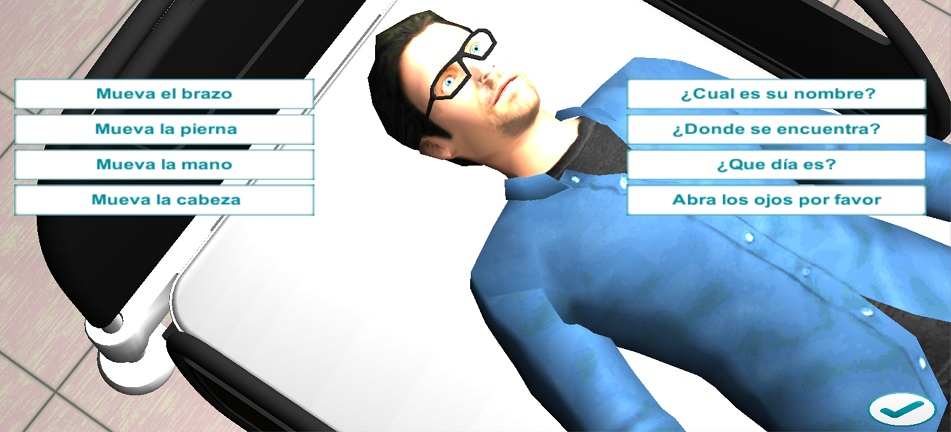
\includegraphics[scale=0.5]{propuesta/glasgow_comandos_voz.jpg}
\caption{Interfaz de la escena \emph{Evaluación de Glasgow}, se observan los
    \emph{comandos de voz}, así como la opción que permite finalizar la escena
    (esquina inferior derecha).}
\label{fig:glasgow_gui}
\end{figure}

Además se ve en la interfaz, al paciente, que es el foco principal de la cámara.

\subsection{Pantalla de resultados}

Al finalizar ambas escenas, se presenta una pantalla de resultados, la cual es
la encargada de mostrar toda la información que fue recabada durante la escena,
esta información incluye los pasos correctos e incorrectos que realizó el
usuario.

\begin{figure}[H]
\centering
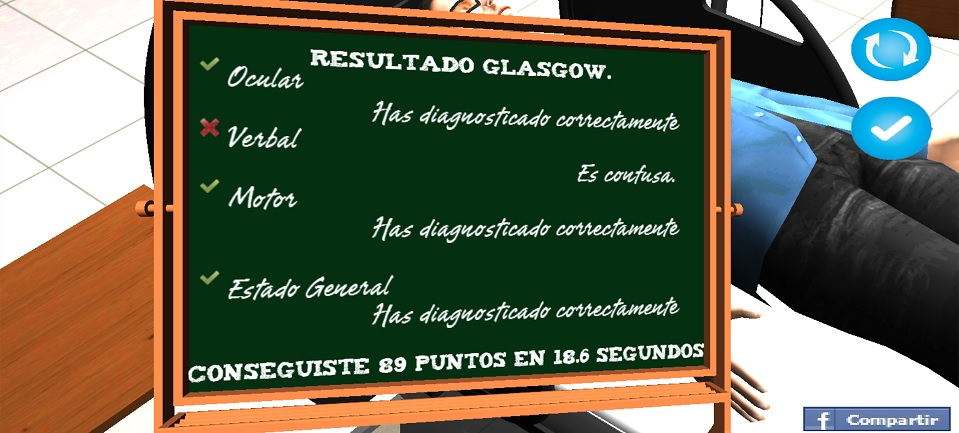
\includegraphics[scale=0.5]{propuesta/resultado_glasgow.jpg}
\caption{Pantalla de resultados mostrando los pasos correctos e incorrectos, en
    la escena \emph{Glasgow}.}
\label{fig:resultados_glasgow}
\end{figure}

Se observa en la figura~\ref{fig:resultados_glasgow} el diseño de la
pantalla, el título es la escena actual, en el pie se observa un resumen de la
puntuación, y el tiempo que duró la escena.

Se lista de manera ordenada los pasos en la parte izquierda de la pantalla, y en
la parte derecha se muestra información relevante acerca del motivo por el cual
no se cumplió cada paso o es caso contrario, se indica que el pao fue realizado 
correctamente.

Adicionalmente a la información de la sesión, se permite al usuario reiniciar la
escena, ir al menú, y compartir sus logros en las redes sociales.

\subsubsection{Retroalimentación}

La retroalimentación se logra a través de la pantalla de resultados, en ella se
presenta información detalla de lo que realizó el usuario. 

Si el usuario realizó de manera incorrecta un paso del procedimiento, esta
información está contenida en una regla (\emph{Extracción de Sangre}), o en el
estado inicial del paciente (\emph{Evaluación de Glasgow}).

\begin{figure}[H]
\centering
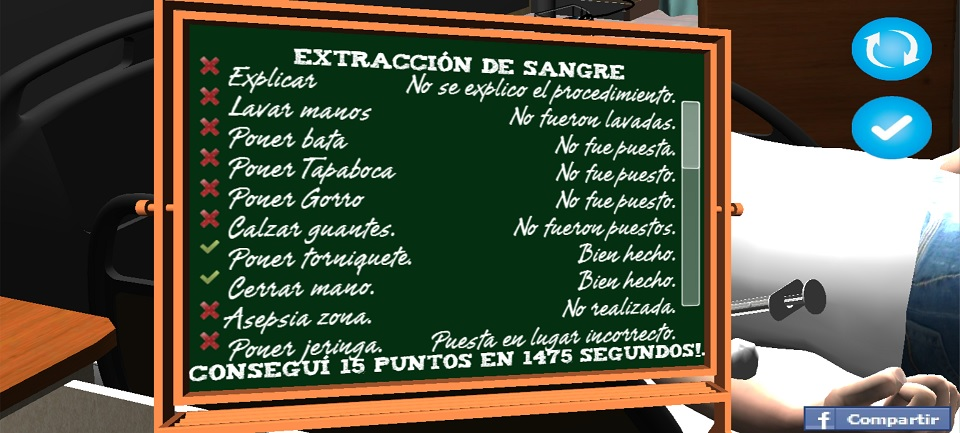
\includegraphics[scale=0.5]{propuesta/resultado_hemocultivo.jpg}
\caption{Pantalla de resultados mostrando los pasos correctos e incorrectos en
    la escena \emph{Extracción de sangre}.}
\label{fig:resultados_hemocultivo}
\end{figure}

Como se observa en la figura~\ref{fig:resultados_hemocultivo}, el paso
\enquote{Poner Jeringa}, contiene la siguiente información \enquote{Puesta en un
    lugar incorrecto}, esto le indica al usuario, que el lugar donde la jeringa
fue insertada era incorrecto, otro posible valor de retroalimentación es
\emph{Jeringa no insertada}.

\subsubsection{Gamificación}

En esta pantalla además se observan opciones que son estudiadas por la
\emph{Gamificación}, entre ellas observamos la puntuación total, el tiempo
utilizado y la utilización de redes sociales.

Si el usuario presiona el botón \enquote{Facebook}, se despliega el menú de
dicha red social, permitiendo que el mismo pueda agregar un mensaje
personalizado y el resultado de la sesión se comparta con el texto \enquote{Conseguí 15 puntos
    en 1475 segundos, en la \emph{Escena Extracción de sangre} jugando con
    YAVE}.


%%! TEX root = ../main.tex
\section{Evaluación en tiempo de ejecución}

Las acciones realizadas por los usuarios dentro de la aplicación son evaluadas para determinar si realizo o no el procedimiento de manera correcta y así brindarle información al usuario sobre su rendimiento.

En esta sección se explica como son evaluados las acciones de los usuarios para los diferentes procedimientos simulados.

\subsection{Extracción de muestras de sangre}

Para la evaluación de las acciones del usuario en este procedimiento se utilizo un motor de reglas denominado "Acciones condicionadas por eventos". A continuación se explica en detalle cada aspecto relacionado tanto al motor como a la forma de evaluación del rendimiento del usuario.

\subsubsection{Acciones condicionadas por eventos}

Un evento es la ocurrencia de un hecho en particular, y son identificados por un
nombre y un conjunto de parámetros, por ejemplo, cuando un evento es cuando el
enfermero inserta una Jeringa, el nombre de este evento es
\emph{''jeringa.inserted''}, y sus parámetros podrían ser el lugar y el tiempo
de la inserción, así, la influencia del estudiante en la simulación es una
sucesión de eventos.

Por cada acción que realiza el usuario dentro de la simulación, existe un evento
relacionado, por consiguiente, es razonable estudiar algunos eventos para
determinar si los pasos realizados corresponden con los deseados. 

Para determinar si una sucesión de eventos es la correcta, se definen reglas,
una regla es una asociación de una condición y una acción, la condición define
si el entorno es el adecuado para realizar una acción, la cual es un
procedimiento que realiza la lógica deseada.

Las \gls{eca} son aquellas que son activadas una vez que se cumplen determinados
eventos\cite{bailey2004event}. En las bases de datos relacionales, son conocidos
como triggers, es decir, una base de datos relacional (u orientada a objetos) es
un motor de reglas \gls{eca}\cite{bailey2004event}\cite{behrends2006combining}.

Las mismas pueden ser utilizadas para notificar que un determinado conjunto de
eventos ha ocurrido\cite{bailey2004event}, así como servir para almacenar
información acerca de la utilización de un determinado recurso.


\paragraph{Motivación}

Las reglas del tipo \gls{eca} permiten reaccionar a determinados eventos, en
forma de una única regla, la cual facilita la declaración de las
mismas\cite{bailey2004event}.

Son principalmente útiles para analizar el comportamiento en tiempo real de un
sistema en una forma
reactiva\cite{bailey2004event}\cite{de2001eca}\cite{bailey2002analysis}, esta
característica esta impulsada principalmente por que son ejecutadas después de
la ocurrencia de un evento, y el entorno no es modificado, pudiendo así acceder
al mismo entorno que el qué lanzo el evento.

Definir si las acciones de un usuario son correctas utilizando un motor
\gls{eca} es sencillo desde el punto de vista que sólo se deben definir un
conjunto de acciones que se deben realizar, y agregar una acción que verifica si
los pasos realizados fueron los correctos.

\paragraph{Declaración}

Una \gls{eca}, se define como\cite{bailey2004event}\cite{behrends2006combining}:

\begin{center}
	 Cuando ocurren una serie de \emph{eventos}, y se cumple una
	 \emph{condición}, entonces realizar una \emph{Acción}.
\end{center}

Los \emph{eventos} determinan cuando una regla debe ser activada, los mismos se
dividen en dos categorías\cite{behrends2006combining}, primitivos y compuestos,
los primeros son detectables, por ejemplo, cuando se inserta una jeringa, y los
compuestos, son la combinación de uno o más
primitivos\cite{bailey2004event}\cite{behrends2006combining}. Los eventos
compuestos, se unen mediante:
\begin{enumerate*}[label=\itshape\alph*\upshape)]
\item conjunción (\emph{y}),
\item disyunción (\emph{o}), y
\item secuencia (\emph{entonces}).
\end{enumerate*}
Sin embargo, no siempre son necesarios todas las posibles combinaciones, y las
combinaciones sencillas son más fáciles de optimizar y
probar\cite{bailey2004event}.

La \emph{condición} de una regla determina si el entorno es el necesario para que la
regla sea activada, en esta condición el entorno que lanzó el evento esta
disponible.

La \emph{acción} a ejecutar describe la lógica que debe ser ejecutada cuando se han
lanzado los eventos y la condición de la regla se ha cumplido.

\paragraph{Dependencia entre reglas}

Las reglas pueden depender de otras reglas, lo cual se puede ver como que la
finalización de una regla es un evento que otra regla espera para poder ser
activada.

Las reglas pueden agregar información a un contexto compartido por todas las
reglas, de esta manera, se puede pasar parámetros entre distintas reglas, por
ejemplo, la regla \emph{Retirar Torniquete}, depende de la regla \emph{Insertar
Torniquete}, pero debe responder solamente al torniquete que ha activado
la regla de inserción, es decir, el usuario puede extraer varios torniquetes, y
la regla no debe activarse, hasta que se extraiga el torniquete que activo la
primer regla.

Así, la regla \emph{Retirar Torniquete} depende de la regla \emph{Insertar
Torniquete}, y esta relación entre reglas, se da en dos
formas\cite{bailey2004event}:

\begin{itemize}
\item  \emph{Dependencia fuerte:} la regla \emph{Retirar Torniquete} solamente podrá
	ser elegida para ser lanzada cuando la regla \emph{Insertar Torniquete}
	haya sido cumplida.
\item  \emph{Dependencia de contexto}: la regla \emph{Retirar Torniquete} no se
	activará cuando los eventos a los que escucha se terminen, sino cuando
	los eventos a los que escucha sean lanzados con los parámetros adecuados
	(se extraiga el torniquete que lanzo la regla de inserción).
\end{itemize}

\paragraph{Representación}

La definición de las reglas se realiza de la siguiente forma;
\begin{algorithm}[H]
\caption{Creación de regla de verificación de calzado de guantes}
\label{alg:rule:guante}
\lstset{style=sharpc}
\begin{lstlisting}
Rule.New("Regla de verificacion de calzado de guantes").
     When("enfermero.guantes.calzar").
     Then(e => e.Patient.ManosLimpias()).
\end{lstlisting}
\end{algorithm}
%TODO agregar indice de algoritmos

La regla anterior controla que el estudiante ha realizado la acción ``Calzarse
los guantes'', y en ese momento tenga las manos limpias, la variable \emph{e},
es el entorno, y a través de la propiedad \emph{Patient} obtiene el estado del
paciente en ese momento.

\paragraph{Modelo de ejecución}

Para ejecutar un motor de reglas del tipo \gls{eca}, se debe tener en cuenta
principalmente dos factores, 
\begin{enumerate*}[label=\itshape\alph*\upshape)]
\item  Como se verifica el cumplimiento de cada regla, y, 
\item  Que ocurre cuando varias reglas son lanzadas al mismo tiempo
\end{enumerate*}.

Para ambos casos se puede tomar un enfoque \emph{inmediato}, es decir que
inmediatamente cuando se lanza un evento, o se cumple una condición, se ejecuta
la regla. Además existen otros dos modos de ejecución, \emph{deferida}, y
\emph{desacoplada}, en la primera, se espera hasta que el lanzador del evento
culmine su trabajo, y luego se ejecuta la regla, pero en la misma unidad de
trabajo, mientras que en la ejecución desacoplada, se encolan los trabajos y
otro hilo es el encargado de ejecutar las reglas. Estos modos están inspirados
en las bases de datos relacionales, el deferido se ejecuta en la misma
transacción, y el desacoplado, inmediatamente después de que la transacción
termine\cite{bailey2004event}.

La propuesta implementada, utiliza una ejecución inmediata, principalmente por
la sencillez de las reglas, es decir, las reglas no realizar un proceso complejo,
solamente controlan el estado del entorno y lo validan.

Además, la ejecución inmediata es importante por que el entorno no sufre
modificaciones entre el evento lanzado y la ejecución de la regla, según
\cite{bailey2004event}, este es el factor más importante para determinar el tipo
de ejecución deseado.



\paragraph{Estados de una regla}

Una regla puede estar en uno de los siguientes estados:

\begin{description}
\item[BEGIN] Es una regla que recién fue creada, no realiza ninguna
	acción.
\item[WAITING\_FOR\_RULE] Es un estado en el que esta esperando que otras reglas
	sean lanzadas. En este estado, es un suscriptor de las reglas por la que
	espera, y no forma parte del ciclo de ejecución del motor de reglas.
\item[WAITING\_FOR\_EVENT] Es un estado en el que esta escuchando a que sean
	lanzados los eventos a los que escucha, este es el estado principal. En
	este estado, es un suscriptor de los eventos por los que espera, y no
	forma parte del ciclo de ejecución del motor de reglas. Se diferencia
	del estado anterior, en que los eventos escuchados pueden ser lanzados
	por cualquier objeto del entorno, no necesariamente una regla.
\item[WAITING\_FOR\_CONDITION] La regla ya no espera por ningún evento y las
	reglas de las que depende ya han sido lanzadas, se verifica cada cierto
	tiempo si el entorno cumple con una condición definida. 
\item[FINISH] La regla ha sido lanzada, con un resultado no determinado, se pudo
	haber cumplido, como no, es el estado final de una regla. Cuando una
	regla llega a este estado, se lanza su evento de finalización.
\end{description}

Una regla puede estar en solo un estado, y solamente se permite que el estado
avance, desde \emph{BEGIN} hasta \emph{FINISH}.


\paragraph{Ciclo de vida}

Cuando una regla es definida, y insertada al motor de reglas, inmediatamente
pasa al estado \emph{BEGIN}, luego se verifica si la misma depende de otras
reglas, sí este es el caso, pasa al estado \emph{WAITING\_FOR\_RULE} y escucha a
los eventos de finalización de las reglas anteriores.

Una vez que las reglas anteriores han sido finalizadas, la regla pasa al estado
\emph{WAITING\_FOR\_EVENT} sí deben escuchar por algún evento, en caso contrario
pasan al estado \emph{WAITING\_FOR\_CONDITION}.

Una vez que la regla está en estado \emph{WAITING\_FOR\_CONDITION}, pasa a un
motor que ejecuta su condición cada cierto tiempo, si la condición se cumple, la
regla se ejecuta, y la misma pasa a estado \emph{FINISH}, momento en el cual
notifica a las reglas que dependen de ella que ha sido lanzada.

Una vez que la regla esta en estado \emph{FINISH}, la misma sale del esquema de
ejecución, y solo esta disponible para obtener resultados.

Según el ejemplo de la regla definida en el código\ref{alg:rule:guante}, la
regla al terminar de ser construida pasa a estado \emph{BEGIN}, al no depender
de otras reglas, pasa inmediatamente al estado \emph{WAITING\_FOR\_EVENT},
cuando es lanzado el evento, la regla ejecuta la acción y pasa al estado
\emph{FINISH}.

\paragraph{Motor de ejecución}

Un motor de reglas \gls{eca}, requiere de un proceso que evalúe constantemente
las reglas para verificar si las mismas deben ser lanzadas o
no\cite{bailey2004event}\cite{galton2002two}, este motor puede utilizar el
algoritmo de RETE\cite{de2001eca} para realizar esta verificación, en la
propuesta presentada, la cantidad de reglas definidas, y la no dependencia
circular entre ellas, hace innecesario la implementación de tal
algoritmo\cite{de2001eca}. 

El motor de reglas actúa sobre aquellas reglas en estado
\emph{WAITING\_FOR\_CONDITION} e invoca al procedimiento que se encarga de
validar si la regla puede ser activada (el procedimiento es único por cada
regla), si el mismo determina que la regla puede ser lanzada, el motor ejecuta
la acción de la regla y modifica el estado de la regla a \emph{FINISH}.


\subsubsection{Definición de reglas}

La reglas del procedimiento de extracción de sangre fueron definidas de acuerdo a los pasos requeridos según el protocolo del procedimiento y al orden en el que son requeridos. Es decir, cada paso del protocolo tiene asociado una regla dentro del motor que lo representa y las condiciones asociadas a cada regla están determinadas por el orden en que deben realizarse dentro del protocolo.

Cada regla tiene una o mas condiciones que deben ser cumplidas para que un paso del protocolo realizado se considere correcto.

\subsubsection{Retroalimentación y puntuación final}

Cada regla tiene asociado un peso, de acuerdo a la dificultad de realizar el paso, este peso es utilizado al final de la partida para darle una puntuación al usuario acerca de su 
rendimiento en la partida.

Además, un regla puede quedar en uno de diferentes estados al final de la partida como se mostró anteriormente, cada uno de esos estados posee un significado en el contexto del procedimiento y por lo tanto tiene información asociada para que al final de la partida se muestre una retroalimentación correcta al usuario por paso.

\subsection{Valoración de la escala de Glasgow}

Para la evaluación del rendimiento del usuario en el momento de llevar a cabo el procedimiento de valoración de la escala de Glasgow se tuvo un enfoque completamente diferente al del procedimiento de extracción de muestras
de sangre debido a la naturaleza propia del procedimiento. 

Como se explico anteriormente, el paciente puede estar en ciertos estados específicos dentro de la escala, y además dentro de cada estado reacciona de un forma en particular por lo tanto, al inicio de la partida
un componente interno de la aplicación selecciona de forma aleatoria un estado para el paciente, de forma tal que cada vez que una partida sea jugada no se repitan los estados de forma seguida.

El estado aleatorio del paciente es guardado en una variable que no es modificada hasta que se reinicie la partida. Al final de la partida, la aplicación pide al usuario que valore el estado del paciente que le fue presentado, una vez que el usuario confirme su respuesta la aplicación la compara con el estado guardado y de esta forma puede informar al usuario acerca de su rendimiento en el diagnostico.

Además, cada posible respuesta dada por el usuario contiene información relacionada al contexto del procedimiento y a la situación actual presentada la cual es utilizada como retroalimentación al final de la partida. La puntuación final dada depende de la cantidad de valoraciones correctas dadas por el usuario para la respuesta verbal, motora, ocular y nivel de gravedad del paciente.










\section{Inconvenientes de diseño}

Los mayores inconvenientes de diseño de la aplicación se dieron en el momento de
validar tanto el contenido de la aplicación como la interfaz de usuario, para
sobrellevar estos inconvenientes fueron requeridos la intervención de terceros.

A continuación se explica en detalle cada uno de los casos.

\subsection{Interfaz de usuario}

Como parte del diseño y desarrollo de la solución se realizó una prueba de
interfaz de usuario con alumnos de la carrera de Ingeniería en Informática de la
\Gls{fpuna}, estas pruebas fueron realizadas con personas que están
acostumbradas al uso de interfaces similares y que, de hecho pueden ser mas
criticas a la hora de evaluarlas. Esta prueba se explica en detalle en el
capítulo~\ref{chap:evaluacion} y los resultados en el
capítulo~\ref{chap:analisis}.

Principalmente son dos las cualidades de una interfaz gráfica que se pueden
someter a prueba: la funcionalidad y la usabilidad. Con la primera se pretende
responder preguntas como \textit{¿Se puede usar cierta función?},
\textit{¿Funciona como se espera?}, o \textit{¿Es correcta?}; y con respecto a
al usabilidad, se espera poder responder a \textit{¿Puede el usuario
    utilizar fácilmente la función?}, o \textit{¿Su uso es intuitivo y fácil de
    aprender?}\cite{fragaverificacion}.

Las pruebas de interfaces de usuario ayudan a que los usuarios puedan
concentrarse mas en el problema en vez de poner los esfuerzos en recordar todas
las opciones que ofrece la solución que se utiliza para resolver el
problema\cite{horowitz1993graphical}.

Luego de las pruebas de interfaz de usuario, se hicieron correcciones a los
problemas encontrados en la interfaz, los mayores inconvenientes fueron con
respecto a la usabilidad y la interacción tanto con el entorno como con los
objetos dentro de la simulación. Estas correcciones, como paso posterior, fueron
probadas por profesores de la carrera de enfermería del \Gls{iab} los cuales
dieron su visto bueno.

Otra de las razones por las cual la prueba fue realizada con alumnos que no
formaban parte de la población a la que iba dirigida la aplicación, es la poco
disponibilidad de tiempo con la que cuentan los alumnos de enfermería y mas aún
los profesionales que están encargados de su aprendizaje.

\subsection{Validaciones de contenido}

Llamamos validación de la simulación o la aplicación desarrollada al hecho de
que el contenido de la misma sea correcto y además que la forma de realizar o
representar dicho procedimiento este acorde al mismo. Este tipo de validaciones
fueron realizadas reiteradamente en reuniones con distintos profesores de la
carrera de enfermería del \Gls{iab}.

Cada corrección solicitada fue evaluada y aprobada posteriormente por los
mismos. Como validación final la aplicación fue presentada en totalidad frente a
un plenario de cuatro profesores del instituto.

El mayor inconveniente en cuanto a las validaciones fueron la forma de
representación tanto de la información como de la simulación de objetos.

\section{Backend de la solución}

\subsection{Registro de usuarios}
\subsection{Registro de eventos}

